\documentclass[12pt, oneside]{book} 
\pagestyle{plain}

% The \usepackage{} command will import predefined fonts, symbols, environments, etc.  For example, the ams packages below come from the American Mathematical Society and include all kinds of useful math symbols like integrals
\usepackage{algorithm,algpseudocode}
\usepackage{tabularx}
\usepackage[table]{xcolor}
\usepackage{amscd}
\usepackage{amsmath}
\usepackage{amssymb}
\usepackage{amsthm}
\usepackage{verbatim}
\usepackage[utf8]{inputenc}
\usepackage{geometry}                		% See geometry.pdf to learn the layout options. There are lots.
\geometry{a4paper}                   		% ... or a4paper or a5paper or letterpaper
%\geometry{landscape}                		% Activate for for rotated page geometry
\usepackage[pdftex]{graphicx}				% Use pdf, png, jpg, or eps with pdflatex; use eps in DVI mode	
\usepackage{setspace}
\usepackage{physics}
\usepackage{subcaption}
% \usepackage[numbers]{natbib}
\usepackage{pdfpages}
\usepackage{bm}
\usepackage{wrapfig}				% enables the use of \wrapfig, for figures with text wrapped around them
\usepackage{afterpage}
\newcommand\blankpage{%
    \null
    \thispagestyle{empty}%
    \addtocounter{page}{-1}%
    \newpage}

\usepackage{bibentry} % for list of publications
\usepackage{hyperref} % create hyper link

% \usepackage[english]{babel}
\graphicspath{{images/}{{\subfix{images/}}}}
\usepackage{tikz}
\usepackage{tikz-3dplot}
\usetikzlibrary{shapes,calc,positioning}
\tdplotsetmaincoords{70}{120}
% \usepackage{siunitx}
\usepackage{adjustbox}
% \usepackage{xcolor} %% Text color
\usepackage{blindtext}
\usepackage{subfiles} % Best loaded last in the preamble
\usepackage{multicol,multirow}  %% Figure in two columns
\usepackage{mathtools, nccmath}

\usepackage{lipsum}			% gives access to \lipsum, which dumps some latin text into your document as filler if you want to check formatting

% \usepackage[parfill]{parskip}    		% Activate to begin paragraphs with an empty line rather than an indent
\usepackage{cleveref}

%reference part
% \usepackage{biblatex} %Imports biblatex package
\usepackage[sorting=none]{biblatex}
\addbibresource{mybib.bib} %Import the bibliography file



% Here we set the page dimensions to match the standard thesis format.  These values should not be changed.
%%% SET LENTGH AND WIDTH %%%
\setlength{\textwidth}{6.5in}
\setlength{\textheight}{8.5in}
\setlength{\oddsidemargin}{0pt}
\setlength{\evensidemargin}{0pt}
\setlength{\topmargin}{0pt}
\setlength{\marginparsep}{0pt}
\setlength{\marginparwidth}{1in}

%self new commands settings
\newcommand\setrow[1]{\gdef\rowmac{#1}#1\ignorespaces}
\newcommand\clearrow{\global\let\rowmac\relax}
\algrenewcommand\algorithmicrequire{\textbf{Input:}}
\algrenewcommand\algorithmicensure{\textbf{Output:}}
\newcommand{\taninv}{\tan^{-1}}

%set up line spacing for the whole document
% \doublespacing
\onehalfspacing
%In order to make a part of the text of your document singlespaced, you can put:
% \begin{singlespace}
% at the beginning of the text you want singlespaced, and
% \end{singlespace}

%\begin{document} starts LaTeX looking for actual content.  Everything above this point is purely formatting.
\begin{document}

%set up title page
\begin{titlepage}
  \begin{center}

    % logo
    \begin{figure}
      % \vspace*{-4cm}
      \hspace*{-0.7cm}
      \centering
      
\includegraphics[scale=0.5]{figures/Nagoya_Logo.png}
      \vspace{0.8cm}
    \end{figure}

    % \vspace* creates some vertical white space on the page to make the title page look more pleasing.  \vspace would do much the same thing, but would not insert the white space if we were at the top of a fresh page.  As this is the start of the document we're obviously at the beginning of a page, so the asterisk is necessary to ensure we still put in two cm of white space.
    \vspace*{2cm}

    {\Large \textbf{Development of Human Following Mobile Robot System with 3D LiDAR and Online Human Classifier}} % \huge sets the font size.  Other options include things like \large, \Large, \small, \tiny, etc.

    \vspace*{2cm}
    { Thesis submitted to the undergraduate degree program in G30 Automotive Mechanical Engineering, Department of Mechanical and Aerospace Engineering and G30 Undergraduate faculty of Nagoya University in partial fulfillment of the requirements for the degree of Bachelor of Engineering.}

    \vspace*{2cm}
    {\large \textbf{Le Nhat Quang}}

    % \vspace{0.5cm}

    {\large \textbf{081851013}}

    \vspace*{1cm}

    {\large \textbf{Supervised by Prof. Naoki Akai and Prof. Susumu Hara}}

    \vspace*{2.0cm}

    {\large Hara laboratory of Control Systems Engineering}

    % \vspace{0.5cm}

    % \begin{comment}
    % {\large Autonomous Robots and Intelligent Control (ARIC) group}
    % Please erase this since this is not official
    % \end{comment}

    % \vfill creates an arbitrary amount of vertical white space as necessary to fill the page
    \vfill

    July 2022

    % \vspace*{3cm}

  \end{center}
\end{titlepage}

% \frontmatter defines the pieces of the thesis which will use roman numerals for page numbering
% \frontmatter 

% The \mainmatter command defines the main body of the thesis and indicates where regular numbering starts
% \mainmatter
\mainmatter


% \chapter{} and/or \chapter*{} will create a chapter in your thesis.  Including the asterisk will cause the chapter to not appear in the table of contents.

\afterpage{\blankpage}

%\tableofcontents will create a table of contents.  By default it will include entries for any \chapter, \section, and \subsection command that appears in your thesis unless you have called the tag with an asterisk
% \tableofcontents

\begin{singlespace}
  \tableofcontents
\end{singlespace}

% \chapter*{Dedication}
% Here a space for dedications...
% \afterpage{\blankpage}

% \chapter*{Abstract}
% % The abstract includes a summary of the main ideas developed in your dissertation. This section is the first one that is part of the main document and can be included with the \textit{$\backslash$input} command in the file \textbf{MainDocuments.tex}. To start a document, no tags are need. You can start writing straight away.

Human-following robots have emerged as a hot research topic in a variety of mobile robotics and computer vision applications because they have many practical applications such as personal airport guides, autonomous cars and surveillance systems. Human following is one of the most essential capabilities of mobile robots in human–robot interaction. Apart from apparent safety considerations, differentiating between humans and inanimate items gives additional information for the robot to plan and modify its future movement in the surroundings. To efficiently follow a specific person, the robot must be able to detect the target individual person within the surrounding indoor environment. In order to recognize human, numerous methods have been proposed such as RGB and RGB-D cameras and 2D LiDAR. Although the application of 3D LiDAR sensors in robotics field has also increased recently, there are still not so many researches has been conducted on 3D LiDAR-based human detection compared to that of RGB-D camera and 2D LiDAR. Moreover, human recognition in 3D LiDAR scans still remains difficult, particularly when the human is too close or too far away from the robot. Working with 3D LiDAR also presents the problem of detecting humans from a sparse number of points and without extra color information. Also, there is currently a lack of human dataset and model that make the classification part is tedious, especially when many variations of human pose, shape and size needed to be classified. 

In this thesis, based on many other previous researches, a pipeline to detect human in indoor environment will be proposed. In addition, planning and control system will also be integrated to make the mobile robot follow a specific person in that environment. Specifically, iCart-mini robot will be equipped with Velodyne VLP-16 3D LiDAR to detect and follow human. The pipeline will consist of several stages, including using 3D SLAM algorithms for synchronizing the raw data point cloud obtained from the LiDAR, ground detection and clustering. For the classification section, a online learning SVM-based method will be used along with built dataset. The pipeline will be implemented in ROS framework with the help of PCL library. A simulation model of iCart-mini mobile robot with Velodyne LiDAR will be constructed in Gazebo environment for debugging and testing. To navigate the robot to the human’s position, PID controller will be used to reduce the error distance between the robot position and target position. Data obtaining from simulation results will be compared with real experiment data collected in the indoor environment. Final results will be evaluated based on ROC curve and successful tracking rate and computation time. 
% % \afterpage{\blankpage}

% \begin{singlespace}
%   \chapter*{Abstract}
%   % The abstract includes a summary of the main ideas developed in your dissertation. This section is the first one that is part of the main document and can be included with the \textit{$\backslash$input} command in the file \textbf{MainDocuments.tex}. To start a document, no tags are need. You can start writing straight away.

Human-following robots have emerged as a hot research topic in a variety of mobile robotics and computer vision applications because they have many practical applications such as personal airport guides, autonomous cars and surveillance systems. Human following is one of the most essential capabilities of mobile robots in human–robot interaction. Apart from apparent safety considerations, differentiating between humans and inanimate items gives additional information for the robot to plan and modify its future movement in the surroundings. To efficiently follow a specific person, the robot must be able to detect the target individual person within the surrounding indoor environment. In order to recognize human, numerous methods have been proposed such as RGB and RGB-D cameras and 2D LiDAR. Although the application of 3D LiDAR sensors in robotics field has also increased recently, there are still not so many researches has been conducted on 3D LiDAR-based human detection compared to that of RGB-D camera and 2D LiDAR. Moreover, human recognition in 3D LiDAR scans still remains difficult, particularly when the human is too close or too far away from the robot. Working with 3D LiDAR also presents the problem of detecting humans from a sparse number of points and without extra color information. Also, there is currently a lack of human dataset and model that make the classification part is tedious, especially when many variations of human pose, shape and size needed to be classified. 

In this thesis, based on many other previous researches, a pipeline to detect human in indoor environment will be proposed. In addition, planning and control system will also be integrated to make the mobile robot follow a specific person in that environment. Specifically, iCart-mini robot will be equipped with Velodyne VLP-16 3D LiDAR to detect and follow human. The pipeline will consist of several stages, including using 3D SLAM algorithms for synchronizing the raw data point cloud obtained from the LiDAR, ground detection and clustering. For the classification section, a online learning SVM-based method will be used along with built dataset. The pipeline will be implemented in ROS framework with the help of PCL library. A simulation model of iCart-mini mobile robot with Velodyne LiDAR will be constructed in Gazebo environment for debugging and testing. To navigate the robot to the human’s position, PID controller will be used to reduce the error distance between the robot position and target position. Data obtaining from simulation results will be compared with real experiment data collected in the indoor environment. Final results will be evaluated based on ROC curve and successful tracking rate and computation time. 
% \end{singlespace}

% \chapter*{Declaration}
% I hereby declare that this thesis is all my own work, except as indicated or cited in the text. This Bachelor report has been completed by myself independently without outside help and only the defined sources and study aids were used. Sections that reflect the thoughts or works of others are made
known through the definition of sources.

\begin{flushright}
Le Nhat Quang\\
July 2022
\end{flushright}

% \afterpage{\blankpage}

% \chapter{List of Publications}
% 

\section*{Peer-reviewed Journal Publications}
\begin{enumerate}
    \item Estrada-Lugo, H. D., Tolo, S., De Angelis, M., \& Patelli, E. (2019). Pseudo credal networks for inference with probability intervals. ASCE-ASME J Risk and Uncert in Engrg Sys Part B Mech Engrg, 5(4).
    \item Morais, C., Estrada-Lugo, H. D., Tolo, S., Jacques, T., Moura, R., Beer, M., \& Patelli, E. (2022). Robust data-driven human reliability analysis using credal networks. Reliability Engineering \& System Safety, 218, 107990.
\end{enumerate}


\section*{Peer-reviewed Conference Publications}
\begin{enumerate}
    \item Estrada-Lugo, H. D., De Angelis, M., \& Patelli, E. (2019, May). Probabilistic risk assessment of fire occurrence in residential buildings: Application to the Grenfell Tower. In 13th International Conference on Applications of Statistics and Probability in Civil Engineering.
\end{enumerate}

% Alternatively you can use the \nobibliography command, but for some reason it gives me an error. 
% \nobibliography{bibliography}
% \bibliographystyle{unsrtnat}

% \section*{Peer-reviewed Journal Publications}
% \begin{enumerate}
%     \item \bibentry{sample1}
%     \item \bibentry{sample2}
%     \item \bibentry{sample3}
% \end{enumerate}


% \section*{Peer-reviewed Conference Publications}
% \begin{enumerate}
%     \item \bibentry{sample4}
%     \item \bibentry{sample5}
%     \item \bibentry{sample6}
% \end{enumerate}
% \afterpage{\blankpage}

%list all tables and figures
\listoftables
% \listoffigures

\begin{singlespace}
  \listoffigures
\end{singlespace}

\chapter*{Abbreviations and nomenclature}
%%%%% Independence symbol definition %%%%%

% \textcolor{red}{
% Please remove this section if you do not write any information.
% }

\newcommand\independent{\protect\mathpalette{\protect\independenT}{\perp}}
\def\independenT#1#2{\mathrel{\rlap{$#1#2$}\mkern2mu{#1#2}}} 
%%%%%%%%%%%%%%%%%%%

%%%%% Nomenclature environment %%%%%
\newbox\tempbox
\newenvironment{nomenclature}{%
   \newcommand\entry[2]{%
       \setbox\tempbox\hbox{##1.\quad}
       \hangindent\wd\tempbox\noindent{##1}\quad\ignorespaces##2\par}
       %\section*{NOMENCLATURE}}{\par\addvspace{12pt}}
       \section*{Nomenclature}}{\par\addvspace{12pt}}
%%%%%%%%%%%%%%  

\begin{nomenclature}
    % \entry{$$}{}
    \entry{$LiDAR$}{Light Detection and Ranging}
    \entry{$HFR$}{Human Following Robot}
    \entry{$ROS$}{Robot Operating System}
    \entry{$RANSAC$}{Random Sample Consensus}
    \entry{$P$}{Initial point cloud data}
    \entry{$p_i$}{Point $i$ in point cloud data $P$}
    \entry{$d_t$}{Distance threshold for RANSAC}
    \entry{$P^*$}{Point cloud data $P^* \subset P$ after being filtered by RANSAC}
    \entry{$ROI$}{Region of Interest}
    \entry{$C$}{List of point cloud clusters from $P$}
    \entry{$d^*$}{Clustering threshold}
    \entry{$r$}{Detected range of LiDAR}
    \entry{$\theta$}{LiDAR vertical angle resolution}
    \entry{$SVM$}{Support Vector Machine}
    \entry{$EKF$}{Extended Kalman Filter}
    \entry{$C-SVC$}{C-Support Vector Classification}
    \entry{$RBF$}{Gaussian Radial Basic Function}
    \entry{$TP$}{True Positive}
    \entry{$TN$}{True Negative}
    \entry{$FP$}{False Positive}
    \entry{$FN$}{False Negative}
    \entry{$PID$}{Proportional, Integral and Derivative Control}
    \entry{$Rviz$}{ROS Visualisation}
\end{nomenclature}


%Example%

% \begin{nomenclature}
% 	\entry{$X$}{Random variable.}
% 	\entry{$x_i$}{State $i$ of $X_i$.}
%     \entry{$\Pi_i$}{Variable $X_i$'s parent.}
%     \entry{$\pi_i$}{State $i$ of $X_i$'s parent.}
%     \entry{$m$}{Number of variables in the network}
%     \entry{$n$}{Number of states of a random variable}
%     \entry{$P(\textbf{X})$}{Joint probability distribution.}
%     \entry{$P(x_i)$}{Probability distribution of a random variable $X_i$ in state $x_i$.}
%     \entry{$P(x_i|\pi_i)$}{Probability of child node $x_i$ conditioned to its parent $\pi_i$.}
%     \entry{$x_q$}{Query variable}
%     \entry{$x_e$}{Observed variable (evidence).}
%     \entry{$x^c$}{Complement state}
%     \entry{$\underline{P}(x)$}{Lower bound.}
%     \entry{$\overline{P}(x)$}{Upper bound.}
%     \entry{$\underline{\overline{P}}(x)$}{Interval probability.}
%     \entry{$K(X)$}{Credal set over $X$.}
%     \entry{$ext[K(X)]$}{Extreme point of the credal set $K(X)$.}
%     \entry{$U$}{Universe of random variables in network.}
%     \entry{$A \independent{B}$}{Variable $A$ independent of $B$.}
% \end{nomenclature}




\chapter{Introduction}
\label{Chap:Intro}
% % Type here the introduction to your dissertation. You can create different sections or subsections with the corresponding commands.
% A .tex file can be created (and placed in the Chapter folder) for each chapter and be called in the MainDocument.tex file with the \textit{$\backslash$input} command. This format is handy when doing "collection of papers" type of thesis, as it is easier to add your articles .tex files to this document. 
\section{Research Background}

% \subsection{Next subsection}

The development of robots now plays a very important role in many different fields, such as civil,
medical, educational and so on \cite{intro_1,chapter1-1,}.Society is moving towards the fact that humans can live with robots, with robots
being more and more intelligent to be able to assist people in work as well as in daily life.
The intelligence of the robot is the determining factor of the robot's ability. As robots get smarter,
handling tasks will become easier and smoother.
Thus, the research of artificial intelligence is now very developed.\\

\begin{figure*}[h]
    \centering
    \begin{minipage}{\columnwidth}
        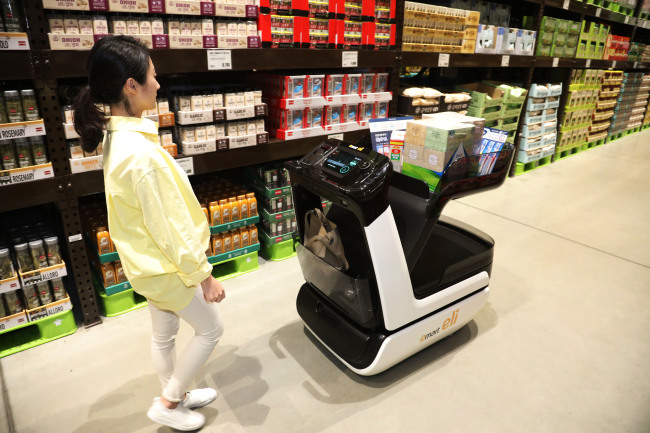
\includegraphics[width=0.48\linewidth]{figures/chap1_fig/20180417000736_0.jpg}
        \hfill
        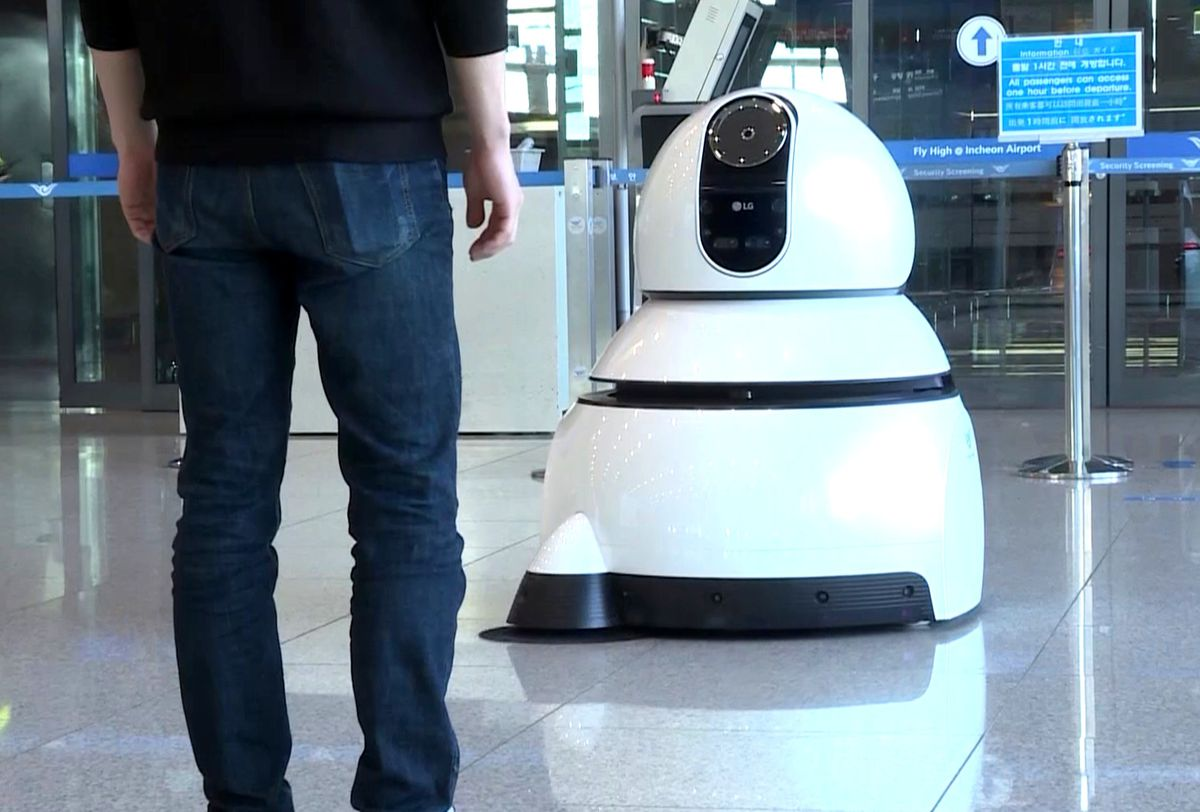
\includegraphics[width=0.48\linewidth]{figures/chap1_fig/Airport_Cleaning_Robot_02.jpg}
        \caption{Application of robot in real life\cite{intro_2,intro_3}}
        \label{Chap1:Fig1}
    \end{minipage}\hfill
\end{figure*}

Examples of applications of robots today are various, notably the application of robots to transport
goods in factories, robot vacuums, or receptionist robots with recognition
technology to assist people at airports or public areas. In addition, there are some robot applications
that follow humans to assist with specific tasks such as carrying luggage or goods (see Fig.~\ref{Chap1:Fig1}).
These systems generally use sensors to recognize information about the external environment, combined with machine learning algorithms to increase accuracy in object recognition and tracking\cite{chapter1-2}.A people following system by a robot is composed of two main modules: people identification and tracking and control to follow a recognized person.\\

\section{Research purpose}

% In this study, the focus will be on the identification and tracking of people. For previous studies, most used
In this research, we focus on identification and tracking of people. For previous studies, most used
2D LiDAR  sensors or cameras. For cameras, there are now many algorithms to identify and track people,
but for complex environments, there are still limitations such as poor visibility in weather conditions, and especially the use of cameras \cite{chapter1-3}. The field of vision is narrow, making it simple to lose the item while following and challenging to catch the right thing in time. % As for the use of 2D LiDAR, it allows identification in a wide range, can track 360 degrees, but following people in complex environments is somewhat limited because the features from 2D LiDAR  are very few, easily confused with other objects.\\
As for the use of 2D LiDAR, it allows identification in a wide range, can track 360 degrees, but following people in complex environments is limited because the features from 2D LiDAR  are very few, easily confused with other objects.\\

% Therefore, in this study, I will use 3D VLP16 LiDAR . Because 3D LiDAR  has a wide scanning range and 360 degrees
In this study, we use 3D VLP16 LiDAR . Because 3D LiDAR  has a wide scanning range and 360 degrees
like 2D LiDAR  and can capture more features like a camera. The contribution of that project is to propose a pipeline
for the robot's human tracking using 3D LiDAR.This pipeline includes two main processing parts that are user
identification online learning and control using PID controller. In addition, the pipeline will be added with
constraints and filters to increase the accuracy of identifying and following people. Moreover, using online
learning in training will boost the learning time and data since the model is continuously  updated during the
run, thereby improving accuracy and reducing data collection time from users.\\

The rest of this thesis is organized as follows.
Chapter 2 summarizes related works.
Chapter 3 presents the Human Following Robot Proposed System.
Chapter 4 details all conducted experiments and describes their results.
Chapter 5 concludes this study and states ideas for future work.
% Chapter 6 expresses the author's acknowledgments.
% Chapter 7 gives all the references used in this thesis.





\chapter{Related research}
\label{Chap:Related_research}
Regarding human-following robots, there has been research on this issue for a long time, outstanding Schlegel {\it et al.} \cite{visionbased} used human color and contour information to conduct tracking. In the study, the characteristic information was based on the color, edges, and texture of the clothes for tracking. For regular RGB images, Li {\it et al.} \cite{detectionbasedcolor} used image segmentation based on shape and color. The exploitation of image color spaces is also studied, including the use of HSV (Hue, Saturation, Value) and D spaces in the RGB-D space of Ren {\it et al.} \cite{realtimetarget}. Based on those two parameters, the study has determined the skeleton of the subject to be monitored. With the development of machine learning, and deep learning today. Detecting people with a camera has become a lot easier. B.X.Chen {\it et al.} \cite{refchap2-fig1} proposed a pipe for following human robot based ROS using camera and CNN to detect and tracking people (see Fig.~\ref{Chap2:Fig1}).\\ 

\begin{figure}[h]
    \centering
    % \hspace*{-8mm}
    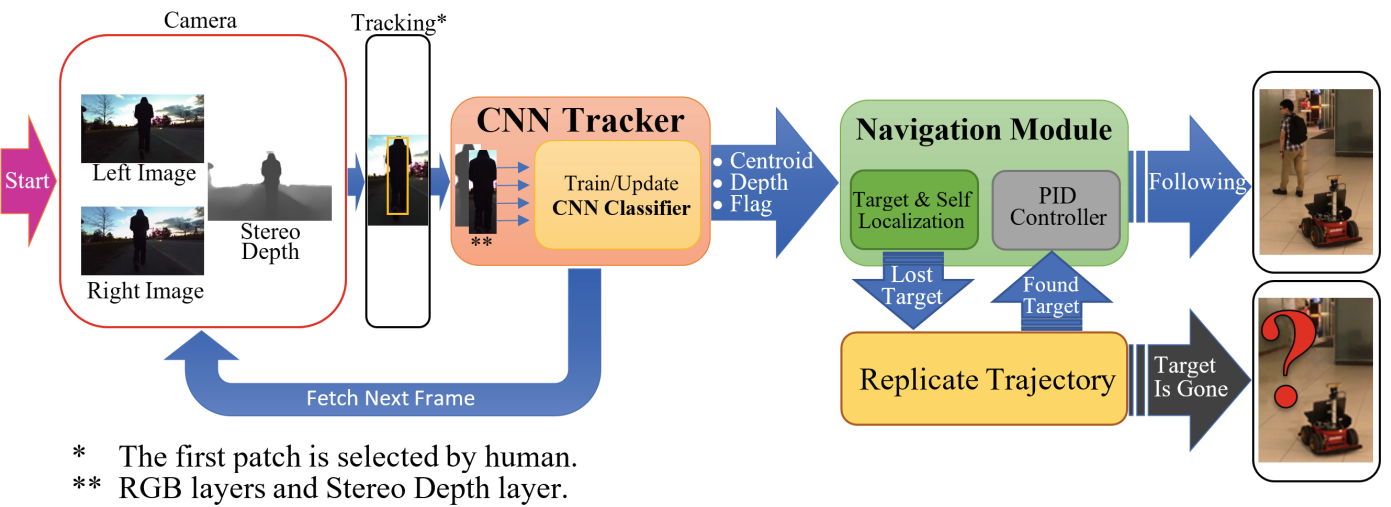
\includegraphics[width=1.0\linewidth]{figures/chap2_fig/pipeline_cnn.png}
    \caption{A Pipeline of the ROS-based Human Following Robot system using camera\cite{refchap2-fig1}}
    \label{Chap2:Fig1}
\end{figure}

In Redhwan.A and Mun-Taek.Ci's study\cite{DL_Color_feature}, the team used SSD (Single Shot Detector) to optimize human detection, combined with extracting color features in HSV space to track objects. Research using LiDAR  to determine the position of the robot as well as the position of the person in the map, as well as to identify obstacles from which it is possible to create a path from the robot position to the human position for the robot to follow.\\
% \textcolor{red}{
% You use of optimize is sometimes wrong. If you have a cost function and you use an answer that minimizes (or maximizes), you can use ``optimize''.
% In the above case, ``improve human detection accuracy'' is better.
% You did not figures in this section. You must refer the figures if you showed them. If not, you have to remove them.
% }

For the use of cameras in human-following robots, the disadvantage is that the camera has a narrow field of view, the distance for good quality is low, and it may be affected in complex environments or bad weather. Therefore, many studies have begun to use LiDAR as an alternative to the camera. Kawarazaki {\it et al.} \cite{hfr_lrs} proposed a method using LiDAR to detect human shins and obstacles around robots (see Fig.~\ref{Chap2:Fig2}). By using geometric constraints, the study was able to determine where the human shin is, thereby determining the human's position relative to the robot. The quality of the algorithm is at a good level in a simple environment. The main disadvantage of this method is that the information obtained by 2D LiDAR  is very little, so it is easy for the algorithm to confuse the human leg with other objects such as the legs of a table, chair or column. So to improve accuracy, people started using 3D LiDAR  to replace 2D LiDAR .\\

\begin{figure*}[h]
    \centering
    \begin{minipage}{\columnwidth}
        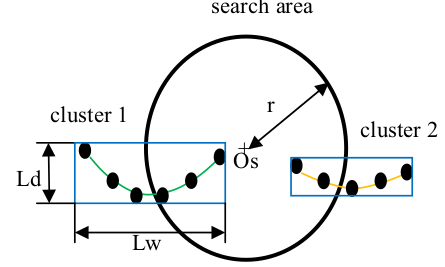
\includegraphics[width=0.48\linewidth]{figures/chap2_fig/shins_human.png}
        \hfill
        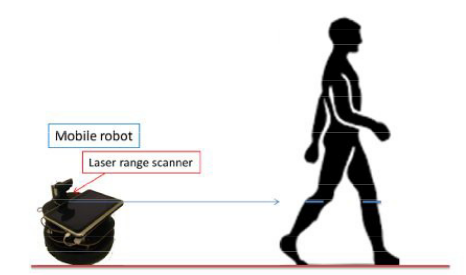
\includegraphics[width=0.48\linewidth]{figures/chap2_fig/shinshuman.png}
        \caption{Shins Human detection and following using LRS\cite{hfr_lrs}}
        \label{Chap2:Fig2}
    \end{minipage}\hfill
\end{figure*}

With 3D LiDAR , the number of point clouds that can scan objects will be much larger than with 2D LiDAR , so one can extract more features from those point clouds. One of the earliest studies on human recognition using 3D LiDAR  was by Luis {\it et al.} \cite{narvano_2009}. Research using Support Vector Machine (SVM) along with seven features. The downside of the study is that it can only detect people standing, not moving, and over short distances. Then in 2011, Kiyosumi Kidono {\it et al.} \cite{kidono}proposed two new features, the Slice feature and the Distributeion of Reflection Intensities. This proposal has somewhat solved the problem of distance and accuracy of detecting people, but there are still disadvantages such as posture or movement of people (see Fig.~\ref{Chap2:Fig3}). To solve those problems, Zhi Yan {\it et al.} \cite{online_learning}has inherited previous studies and added a tracker that helps the algorithm to detect and track moving objects. Removing some features helps to speed up computation. And especially, adding an online learning algorithm has solved the problem of accuracy in detecting people, as well as improving the algorithm when it is possible to continuously update new parameters to increase detection ability. with training time.\\

In light of the benefits and drawbacks of the earlier research approaches, we would like to provide a whole pipeline for the HFR system. The pipeline will contain model changes, user detection and tracking for online learning, input preprocessing (point-cloud), and user detection and tracking for input. We utilize PID as the control method to direct the robot to the person's designated position in the previous phase.

\begin{figure}[h]
    \centering
    % \hspace*{-8mm}
    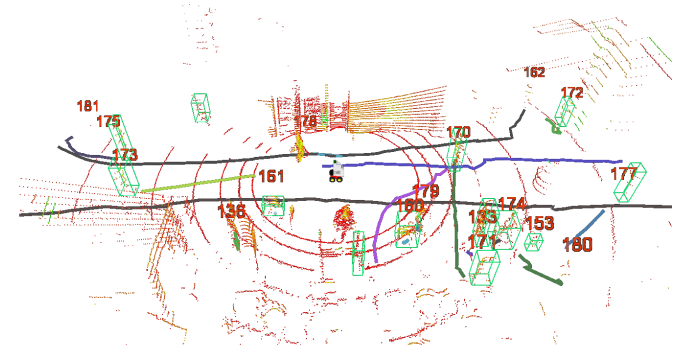
\includegraphics[scale=0.5]{figures/chap2_fig/online_learning.png}
    \caption{Human detection and tracking using Online learning with 3D LiDAR \cite{online_learning}}
    \label{Chap2:Fig3}
\end{figure}


\chapter{Proposed System for Human Following Robot}
\label{Chap:Proposed_system}
%------------3.1--------------------------------------%
\section{Pipeline}
\label{whole_pipeline_intro}

\begin{figure}[h]
    \centering
    % \hspace*{-8mm}
    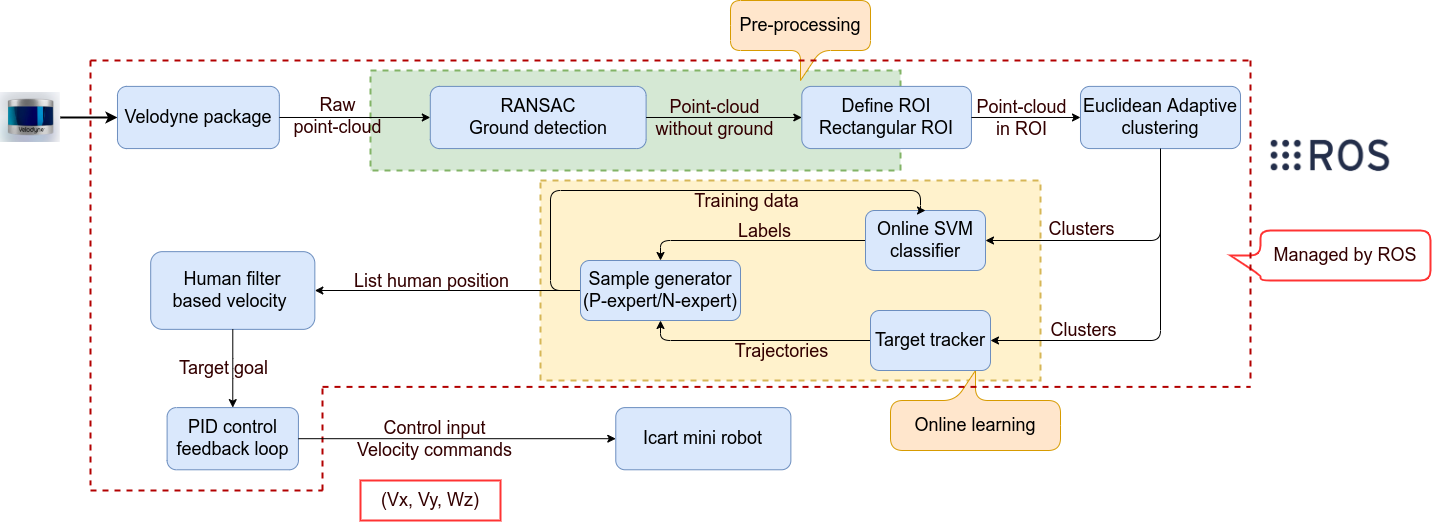
\includegraphics[width=1.0\linewidth]{figures/chap3_fig/pipeline.png}
    \caption{A Pipeline of the ROS-based Human Following Robot system}
    \label{Chap3:Fig1}
\end{figure}

% This section generalizes the proposed pipeline, which is the heart of this thesis.
This section describes the proposed pipeline, which is the heart of this thesis.
This pipeline takes point cloud obtained from a 3D LiDAR onboard an mobile robot as an input
and outputs the final velocity commands for the mobile robot to follow the identified human effectively in
an indoor environment. This pipeline is illustrated as a block diagram in Figure \ref{Chap3:Fig1} above.
The whole process is utterly managed and coded in ROS (Robot Operating System) framework \cite{ros_original}.
In principle, the pipeline can be split into 4 main stages, which are pre-processing step, clustering step,
classification step and control step. The pre-processing step contains RANSAC ground extraction and ROI(Region of Interest) definition,
which is presented in section \ref{pre-processing_step_section}. The clustering step uses Euclidean Adaptive clustering method and is depicted
in section \ref{Euclidean_cluster_section}. Then, section \ref{online_learning_section} describes online learning for SVM(Support Vector Machine) which is the human classification
step. Finally, the control phase is discussed in section \ref{pid_section}, which comprises 2 smaller modules: human filter-based velocity
and PID control feedback loop. The whole pipeline is written in C++ and maintained in author's Github repository.

%------------3.2--------------------------------------%
\section{Pipeline breakdown and details}

%------------3.2.1--------------------------------------%
\subsection{LiDAR point cloud pre-processing step}
\label{pre-processing_step_section}

In this pre-processing step, the ground plane is extracted and removed from the
raw point cloud of Velodyne LiDAR using RANSAC algorithm. RANSAC \cite{ransac} stands for Random Sample
Consensus, which is considered to be a congruous technique to detect and filter out any inliers point cloud
in any set of point clouds using some pre-defined models such as plane model or circle model. RANSAC algorithm used to detect
the plane model is shown in the Algorithm \ref{Chap3:Alg1}. First, the algorithm will select any 3 points in the space randomly to form
a plane. Then, the we evaluate the plane model coefficients $a,b,c,d$ that contains those previous selected points.


\begin{algorithm}[h]
    \caption{RANSAC(Random Sample Consensus) ground plane detection algorithm  \cite{ransac}}
    \label{Chap3:Alg1}
    \begin{algorithmic}[1]
        \Ensure Point cloud data $P^*$ of the plane model
        \Require Point cloud data $P$, where $p_i=[x,y,z] \in P$;
        \State Randomly select three non-collinear unique points $\{p_i, p_j, p_k\}$ from $P$;
        \State Compute the model coefficients from the three points $(ax + by + cz + d = 0)$;
        \State Compute the distances from all $p \in P^* \subset P$ to the plane model $(a,b,c,d)$;
        \State Count the number of points $p^* \in P$ whose distance $d$ to the plane model falls between $0 \leq |d| \leq |d_t|$, where $d_t$ represents a user specified threshold.
    \end{algorithmic}
\end{algorithm}

% \begin{figure}[h]
%     \centering
%     % \hspace*{-8mm}
%     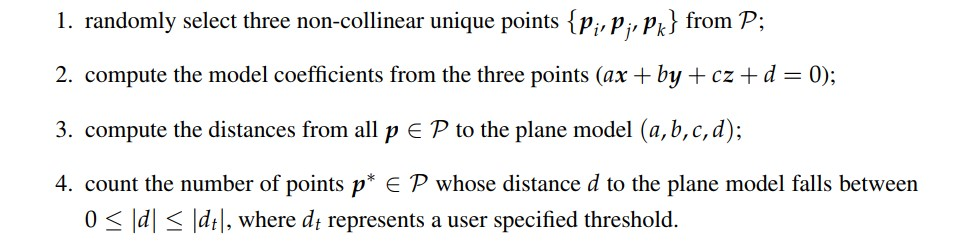
\includegraphics[width=1.0\linewidth]{figures/chap3_fig/preprocess/ransac_algorithm.jpg}
%     \caption{RANSAC(Random Sample Consensus) ground plane detection algorithm \cite{ransac}}
%     \label{Chap3:Fig2}
% \end{figure}


Next, distance from all remaining points is calculated to that plane model, as visualised in Figure \ref{Chap3:Fig3}. A distance
threshold will be set manually and the total number of points whose distances fall within this range will be recorded in each iteration.
This process will be looped until the maximum number of points is reached. For a set of 3D point clouds, especially point clouds captured
in indoor environment such as corridor or in the building, there is a large number of points that will belong to the ground. If those
point clouds are extracted from the set, the next analysis step will be much faster since the computational
time is greatly reduced. Also, filtering out ground point clouds can make the classification step for all points above the ground
plane easier. An example of RANSAC application to extract ground point clouds is shown in Figure \ref{Chap3:Fig4}. When applying
RANSAC, it is assumed that the ground in the experimental environment is completely flat and not rough.

\begin{figure}[h]
    \centering
    % \hspace*{-8mm}
    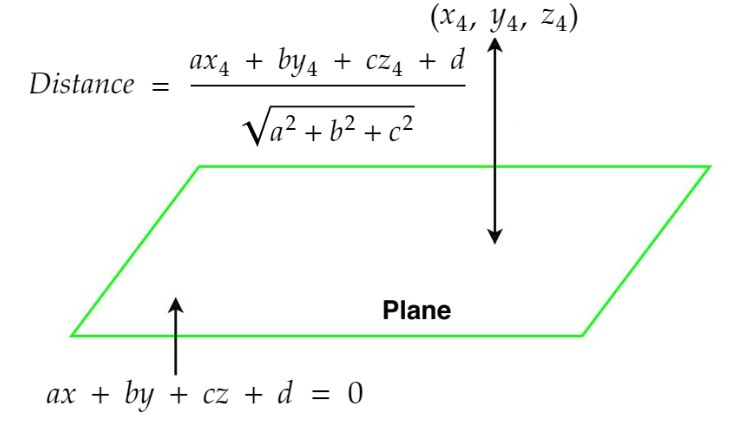
\includegraphics[scale=0.6]{figures/chap3_fig/preprocess/ransac_plane.jpg}
    \caption{RANSAC plane distance estimation \cite{ransac_1}}
    \label{Chap3:Fig3}
\end{figure}

% \clearpage

\begin{figure}[h]
    \centering
    % \hspace*{-8mm}
    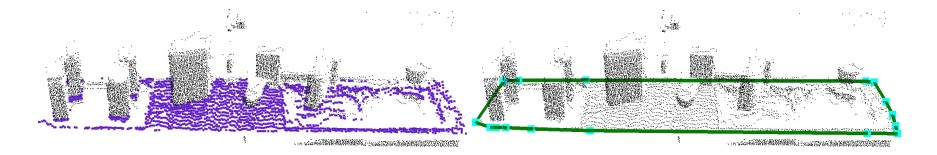
\includegraphics[width=1.0\linewidth,scale=0.8]{figures/chap3_fig/preprocess/ransac_example.jpg}
    \caption{Example of resultant inliers (purple) point support best planar model (ground)  \cite{rusu_thesis}}
    \label{Chap3:Fig4}
\end{figure}

After performing ground segmentation, we need one more small step to accomplish this pre-processing step. Point cloud obtained from
LiDAR scan, after being removed ground points, will be simplified by creating a region of interest(ROI). To put it
differently, we will trim these remaining point cloud by making a box around the mobile robot and get rid of all points outside
this boudary box\cite{cnn_uav}. Robot attached with LiDAR sensor will be the center of this box and in this research, the dimensions
of this box is 10 x 10 x 2m because we want to observe full body of human.


%------------3.2.2--------------------------------------%
\subsection{Adaptive Euclidean clustering}
\label{Euclidean_cluster_section}

In this step,  point cloud that is above the ground and inside a boundary box will be clustered into multiple
separated objects, like the example in Figure \ref{Chap3:Fig5}. This clustering method is known as Euclidean
object clustering technique \cite{rusu_thesis,cnn_uav} and its pseudocode is shown in Algorithm \ref{Chap3:Alg2}.
This method is also regarded as prevalent 3D point cloud analysis technique \cite{3d_pc_analysis}.
This algorithm takes point cloud data P as an input and outputs an array of point cloud clusters C. These
clusters can contain both human and non-human objects that will be fed to the next classification stage.
To implement this algorithm, first kd-tree representation \cite{rusu_thesis} will be created. Array of clusters
C and small set of points Q will be first inilialised, then we will jump into the main loop of Euclidean clustering
method. Point $p_i$ will be added to Q in sequence and in each iteration, another loop is made to search
for any point ${p_i}^k$ within a sphere of radius $r$. This radius is smaller than an assigned threshold
$d^*$. This nested loop will compile until all suitable points are added to Q and Q is added to C. This algorithm
will terminate if all point cloud have been clustered.



\begin{figure}[h]
    \centering
    % \hspace*{-8mm}
    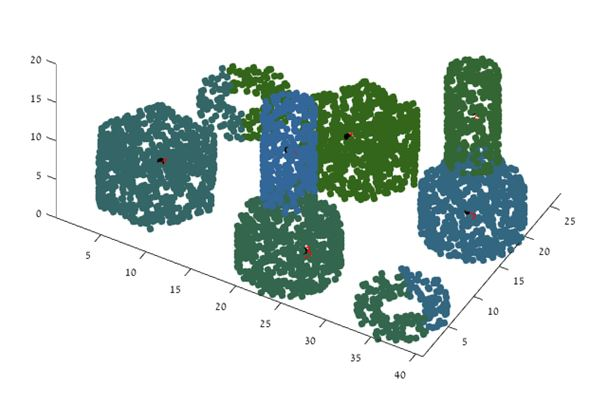
\includegraphics[scale=0.5]{figures/chap3_fig/euclidean/euclidean_example.jpg}
    \caption{Example of Euclidean object clustering  \cite{rusu_thesis}}
    \label{Chap3:Fig5}
\end{figure}

% \begin{figure}[h]
%     \centering
%     % \hspace*{-8mm}
%     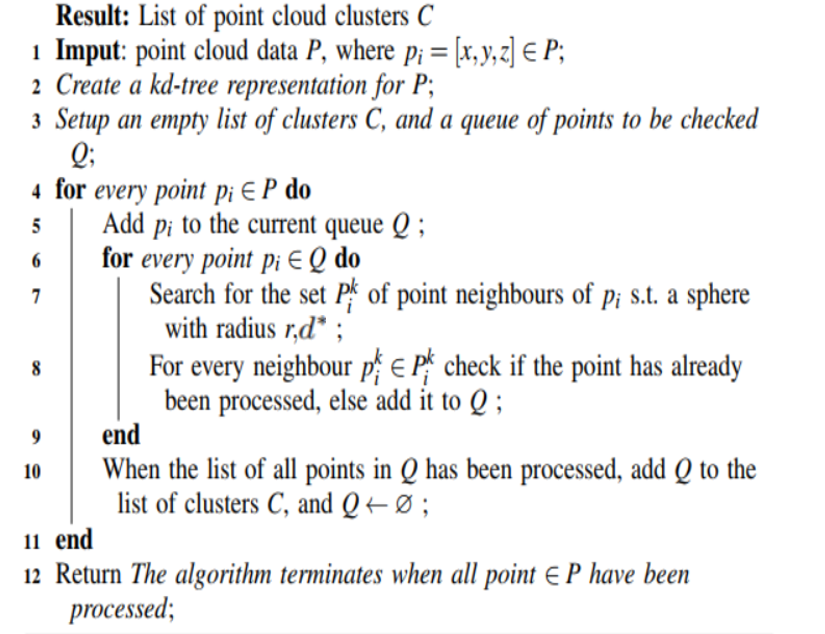
\includegraphics[width=1.0\linewidth]{figures/chap3_fig/euclidean/euclidean_cluster_algorithm.png}
%     \caption{Euclidean clustering algorithm  \cite{rusu_thesis,cnn_uav}}
%     \label{Chap3:Fig6}
% \end{figure}

\begin{algorithm}[h]
    \caption{Euclidean clustering algorithm  \cite{rusu_thesis,cnn_uav}}
    \label{Chap3:Alg2}
    \begin{algorithmic}[1]
        \Ensure List of point cloud clusters C
        \Require Point cloud data $P$, where $p_i=[x,y,z] \in P$;
        \State Create a Kd-tree representation for $P$;
        \State Setup an empty list of clusters $C$, and a queue of points to be checked $Q$;
        \For{every point $p_i \in P$}
        \State Add $p_i$ to the current queue $Q$;
        \For {every point $p_i \in Q$}
        \State Search for the set ${p_i}^k$ of point neighbours of $p_i$ s.t a sphere with radius $r,d^*$
        \State For every neighbour ${p_i}^k \in {p_i}^k$ check if the point has already been processed, else add it to Q;
        \EndFor
        \State When the list of all points in $Q$ has been processed, add $Q$ to the list of clusters $C$, and $Q \gets \emptyset$
        \EndFor
        \State Return the algorithm terminates when all point $\in P$ have been processed;
    \end{algorithmic}
\end{algorithm}

However, although Euclidean algorithm is fast and robust, it has one large disadvantage
that should be taken into account. The hindrance of this method lies in the threshold
$d^*$ parameter. In fact, the accuracy of the clustering result depends predominantly on the the threshold
value. As can be observed in Figure \ref{Chap3:Fig7}, if $d^*$ is too large, point cloud obtained
from some objects can be clustered together. On the contrary, small $d^*$ leads to the consequence
that single target can be divided into multiple clusters. Also, according to \cite{online_learning}, the
human form generated by LiDAR scan varies enormously with respect to the distance between human and LiDAR sensor, as
shown in Figure \ref{Chap3:Fig8} because of LiDAR vertical angular resolution. Thus, we will
tune this threshold value using the scan range of LiDAR \cite{online_learning} using this equation below:

\begin{equation}
    \label{Chap3:Eq1}
    d^* = 2r \tan \frac{\theta}{2}
\end{equation}

In equation \ref{Chap3:Eq1}, r denotes the detected range of LiDAR and $\theta$ is the LiDAR vertical
angle resolution respectively.

\begin{figure}[h]
    \centering
    % \hspace*{-8mm}
    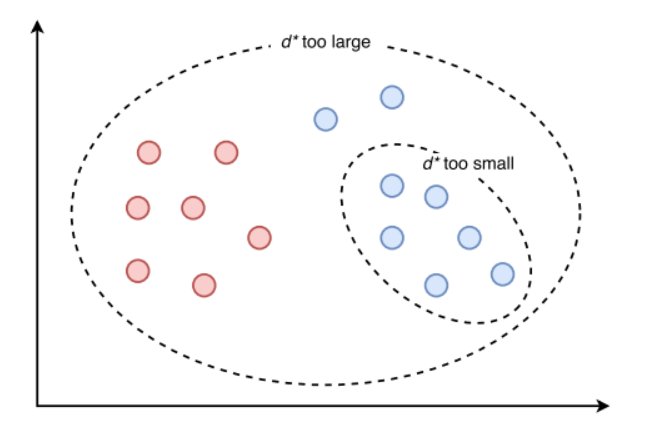
\includegraphics[scale=0.5]{figures/chap3_fig/euclidean/3_2_1.png}
    \caption{Different $d^*$ lead to different clustering results  \cite{online_learning,online_learning_2020}}
    \label{Chap3:Fig7}
\end{figure}

\begin{figure}[h]
    \centering
    % \hspace*{-8mm}
    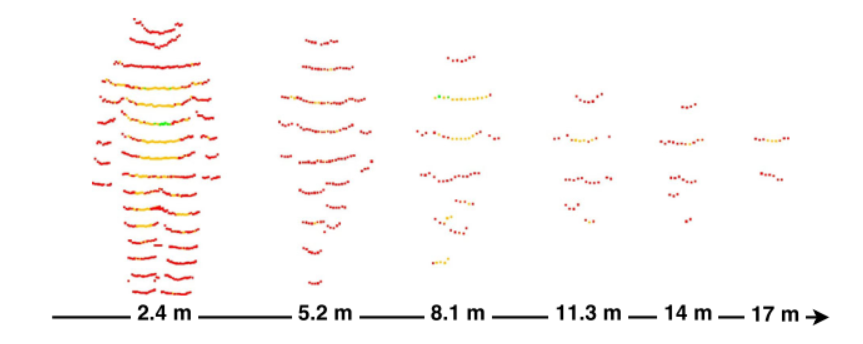
\includegraphics[width=1.0\linewidth]{figures/chap3_fig/euclidean/3_2_2.png}
    \caption{Shape of human point clouds with respect to distance from LiDAR  \cite{online_learning,online_learning_2020}}
    \label{Chap3:Fig8}
\end{figure}

Accordingly for different detection range of LiDAR, an appropriate threshold value
will be determined to make the final clustering result more precise compared to the
traditional Euclidean method. The result of this clustering step will be shown in section
\ref{cluster_result} in Chapter \ref{Chap:ExperimentSetup_Results} below.

% \begin{figure}[h]
%     \centering
%     % \hspace*{-8mm}
%     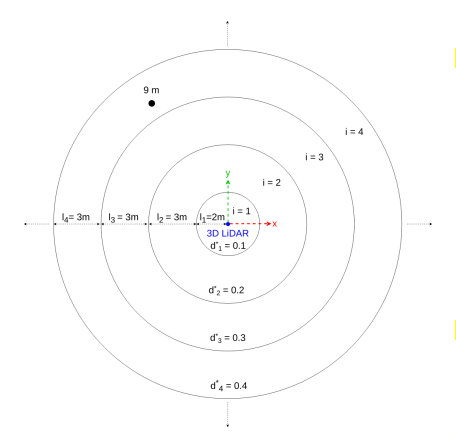
\includegraphics[scale = 1.0]{figures/chap3_fig/euclidean/3_2_3.png}
%     \caption{Values of $d^*$ for various regions \cite{online_learning_2020,online_learning}}
%     \label{Chap3:Fig9}
% \end{figure}

% \begin{figure}[h]
%     \centering
%     % \hspace*{-8mm}
%     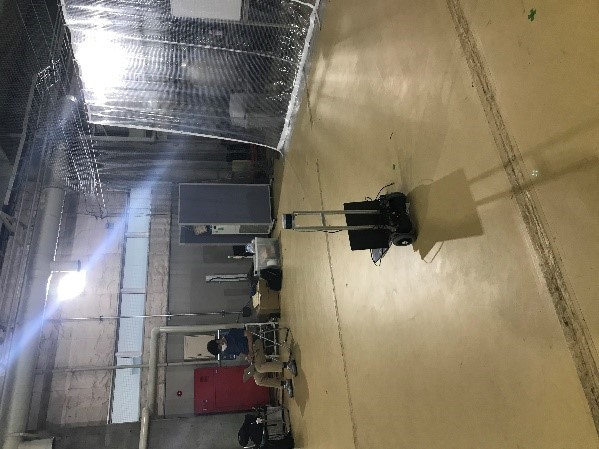
\includegraphics[width=1.0\linewidth,angle = -90]{figures/chap3_fig/euclidean/3_2_4.jpg}
%     \caption{Testing hall}
%     \label{Chap3:Fig10}
% \end{figure}

% \begin{figure}[h]
%     \centering
%     % \hspace*{-8mm}
%     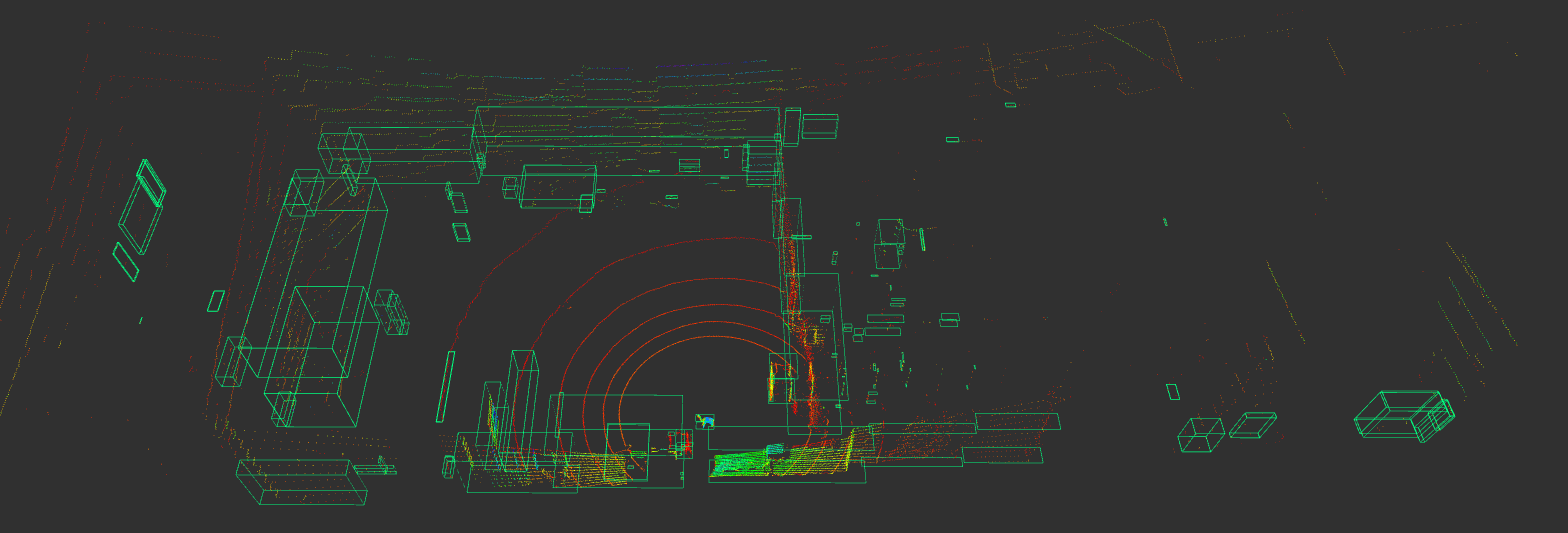
\includegraphics[width=1.0\linewidth]{figures/chap3_fig/euclidean/3_2_5.png}
%     \caption{Testing hall result}
%     \label{Chap3:Fig11}
% \end{figure}

% \begin{figure}[h]
%     \centering
%     % \hspace*{-8mm}
%     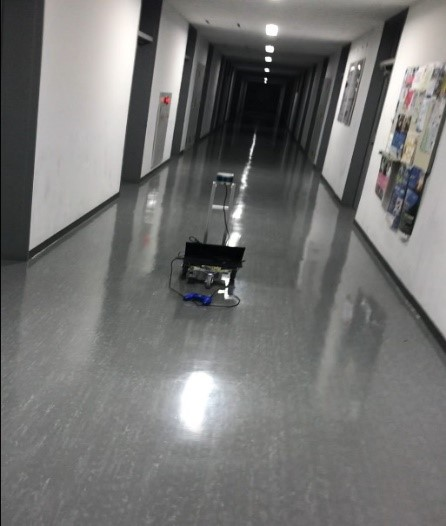
\includegraphics[width=1.0\linewidth]{figures/chap3_fig/euclidean/3_2_6.jpg}
%     \caption{Corridor environment}
%     \label{Chap3:Fig12}
% \end{figure}


% \begin{figure}[h]
%     \centering
%     % \hspace*{-8mm}
%     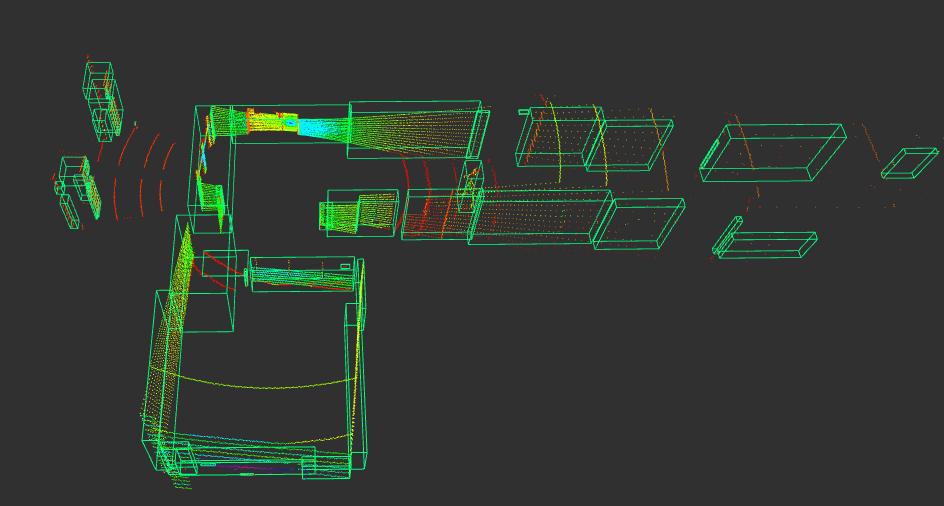
\includegraphics[width=1.0\linewidth]{figures/chap3_fig/euclidean/3_2_7.png}
%     \caption{Corridor environment test}
%     \label{Chap3:Fig13}
% \end{figure}


%------------3.2.3--------------------------------------%
\subsection{Online learning for SVM human classification }
\label{online_learning_section}

The online learning for SVM human classification method which is the most crucial
component of the entire system will be described and analyzed in this section. Figure
\ref{Chap3:Fig14} shows the framework of this learning framework. In short, online learning
process can be broken into 3 parts: the multi-target tracker, human SVM classifier and
P-N sample generator \cite{online_learning}.


\begin{figure}[h]
    \centering
    % \hspace*{-8mm}
    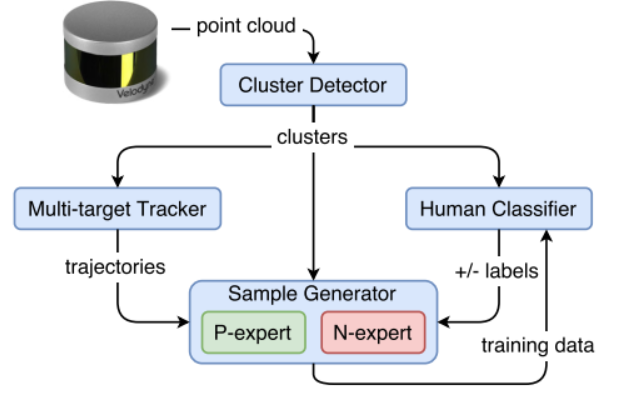
\includegraphics[scale=0.6]{figures/chap3_fig/onlineSVM/3_3_1.png}
    \caption{Online learning framework \cite{online_learning_2020}}
    \label{Chap3:Fig14}
\end{figure}

Each of these part has its own task to complete this online process. The tracker component
estimates the position of each cluster in real time and yields all cluster's trajectories.
Concurrently, the classifier will do its work - classifies whether the cluster is human or
non-human based on the model trained by SVM method. However, the model is not static, it will
be updated continuously with the support from the sample generator. This sample generator
will be the judge in this scenario. In specific, it will correct positive and negative
samples by employing clusters' trajectories information obtained from the tracker and produces
new training data for SVM algorithm. The classifier will be retrained again until some terminating
conditions are satisfied.

The procedure briefly described above is eminently propitious when handling datasets which
are intricate to gather such as human 3D point cloud dataset. Human often has various poses
and different characteristics such as height, body thickness and so on. For that reason, collecting
human datasets for training is considered as tough work and normally requires much efforts to make
good datasets. However, since some features such as point cloud's reflection intensity are completely
distinct, using open-source dataset which is already available on the Internet, namely KITTI is
not appropriate. Thus, batch-incremental training \cite{online_learning,online_learning_2020} as in
Figure \ref{Chap3:Fig14} is effective because new human data is collected online when conducting the
experiment.

EKF (Extended Kalman Filter) and NN(Nearest neighbor) data association \cite{online_learning,online_learning_2020,probab_robot}
are utilised for the cluster tracking process. Although the data obtained is three-dimensional,
only 2D data (i.e x and y coordinates) is used for the tracking. So in this tracking algorithm,
human is supposed to move on a flat plane which should be correct in most indoor environment.
To use EKF, 2 models including velocity model and obseravtion model will be built. The method is much similar
to the traditional Kalman filter, the only difference here is to first linearise all models.
Once the cluster is detected and observed, new cluster states are updated using the polar obseravtion model.
NN data association will be exploited to operate several perceived clusters simultaneously so that all EKFs are
updated in synchronicity \cite{online_learning,online_learning_2020}.

LIBSVM \cite{libsvm} is used to implement the human classifier part of the framework. For this classification task, each human training data has one label and 62 features. The class label can be either 1 (human)
or -1(non-human) and all features using to train the human SVM model are shown in Table \ref{Chap3:Table1} below. The purpose
of SVM is to generate a model that can predict the label of input data, to classify whether this cluster is human or not using
only cluster's features information. We add one more feature $f_3$ or cluster volume, compared to 61 features in \cite{online_learning}.

\begin{table}[h!]
    \centering
    \begin{tabular}{||c|c|c||}
        \hline
        \rowcolor{lightgray}
        \textbf{Feature} & \textbf{Description}                                & \textbf{Dimension} \\ [0.5ex]
        \hline\hline
        $f_1$            & Number of points in cluster                         & 1                  \\
        $f_2$            & Minimum cluster distance from LiDAR                 & 1                  \\
        $f_3$            & Cluster volume                                      & 1                  \\
        $f_4$            & 3D covariance matrix of cluster                     & 6                  \\
        $f_5$            & Normalized moment of inertia tensor                 & 6                  \\
        $f_6$            & Slice feature of the cluster                        & 20                 \\
        $f_7$            & Reflection intensity's distribution (mean, std dev) & 27                 \\ [0.5ex]
        \hline
    \end{tabular}
    \caption{All features for human classification}
    \label{Chap3:Table1}
\end{table}

In this step, C-SVC (C-Support Vector Classification) of LIBSVM is used. The mathematical concept of C-SVC is
constructed as in \cite{libsvm,guide_svm}. For $x_i \in {\mathbb{R}}^{n}$ and output label vector $y_i \in \{ 1,-1 \}$,
C-SVC optimizes this problem:

\begin{equation}
    \label{Chap3:Eq2}
    \begin{split}
        \min_{\alpha}\quad & \frac{1}{2}{\alpha}^{T}Q \alpha - e^T\alpha \\
        \text{subject to } \quad & y^T \alpha = 0 \\
        \text{with } \quad &  0 \leq {\alpha}_i \leq C, i = \{ 1,2,..,62\}
    \end{split}
\end{equation}

% \begin{align*}
%     \min_{\alpha}\quad      & \frac{1}{2}{\alpha}^{T}Q \alpha - e^T\alpha \\
%     \text{subject to }\quad & y^T \alpha = 0                              \\
%     \text{with }  \quad     & 0 \leq {\alpha}_i \leq C, i = \{ 1,2 \}
% \end{align*}

In equation \ref{Chap3:Eq2}, $e$ is vector of all 1 and Q is 62x62 matrix with
$Q_{ij} = y_i y_j K(x_i,x_j)$ . K is defined as kernel function with  $K(x_i,y_j) = {\phi (x_i)}^T \phi (x_j)$ \cite{libsvm,guide_svm}.
There are several kernel functions has been defined such as linear, polynomoial, radial basis function (RBF)
and sigmoid. Among of them, \cite{guide_svm} proposed that RBF kernel should be used. Thus, in
this research, the following kernel function will be used:

\begin{equation}
    K(x_i,y_j) = e^{- \gamma {\|x_i -y_j \|}^2}
\end{equation}

where $C$ and $\gamma$ are 2 parameters which are tuned beforehand.

The sample generator in Figure \ref{Chap3:Fig14} consists P-expert and N-expert. The relation between testing and
real human data is shown in Figure \ref{Chap3:Fig16} below.

% \begin{figure}[h]
%     \centering
%     % \hspace*{-8mm}
%     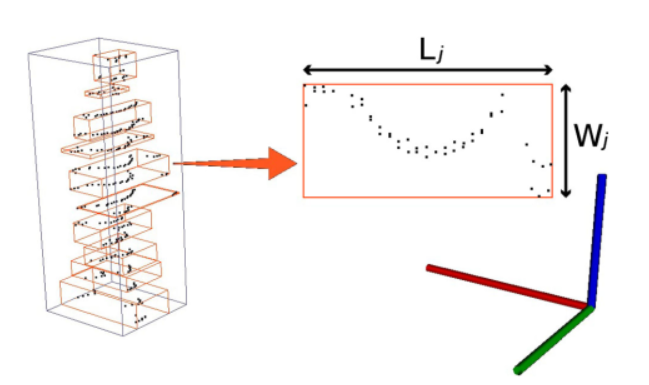
\includegraphics[width=1.0\linewidth]{figures/chap3_fig/onlineSVM/3_3_2.png}
%     \caption{Example of the slice feature \cite{kidono,online_learning_2020}}
%     \label{Chap3:Fig15}
% \end{figure}

\begin{figure}[h]
    \centering
    % \hspace*{-8mm}
    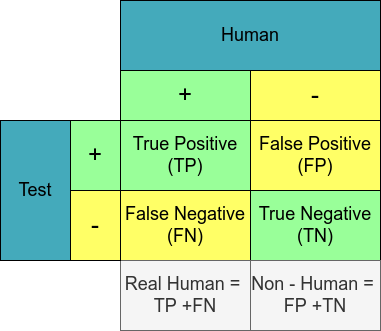
\includegraphics[scale=0.7]{figures/chap3_fig/onlineSVM/TN_FN.png}
    \caption{Positive and Negative clusters}
    \label{Chap3:Fig16}
\end{figure}

From Figure \ref{Chap3:Fig16}, real human clusters are defined as the sum of TP (True Positive) samples and
FN (False Negative) while non-human clusters are the total of FP(False Positive) and TN(True Negative). Evidently,
FN and FP are only 2 cases that must be reduced if we want better classification accuracy. That is where the role of
the sample generator takes place. In specific, all clusters which are categorised as negative samples
are fed to the P-expert of the generator, then this P-expert will assess FN samples and renovate them to positive samples.
Similarly, all clusters which are considered as postive samples in the initial training are fed to the
N-expert and only FP will be transform into negative samples.  This new augmented training data will be
exploited to retrain the whole human classifier \cite{online_learning}. The way P-expert and N-expert
filters out FN and FP samples respectively is genuinely simple. P-expert relies on human-like
trajectory whereas N-expert is governed by approximate static objects. In short, there will be some variances conditions
that have to be satisfied to be considered whether is is human-like or static samples \cite{online_learning}. The
training result will be shown in section \ref{online_svm_result}.



% \textcolor{red}{
% Fig.~\ref{Chap3:Fig16} is too big.
% How you make figures? Vector style figures are preferable more than bitmap ones.
% }


% \begin{figure}[h]
%     \centering
%     % \hspace*{-8mm}
%     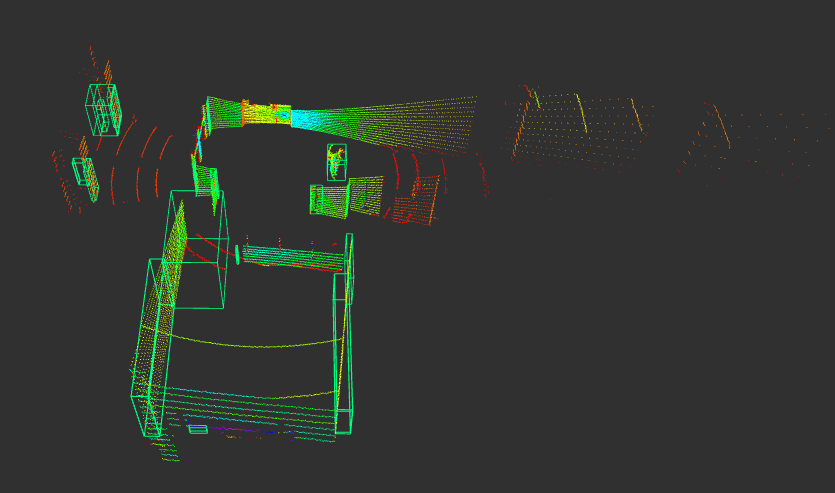
\includegraphics[width=1.0\linewidth]{figures/chap3_fig/onlineSVM/online_train_round1.png}
%     \caption{Online train round 1 (initial)}
%     \label{Chap3:Fig17}
% \end{figure}

% \begin{figure}[h]
%     \centering
%     % \hspace*{-8mm}
%     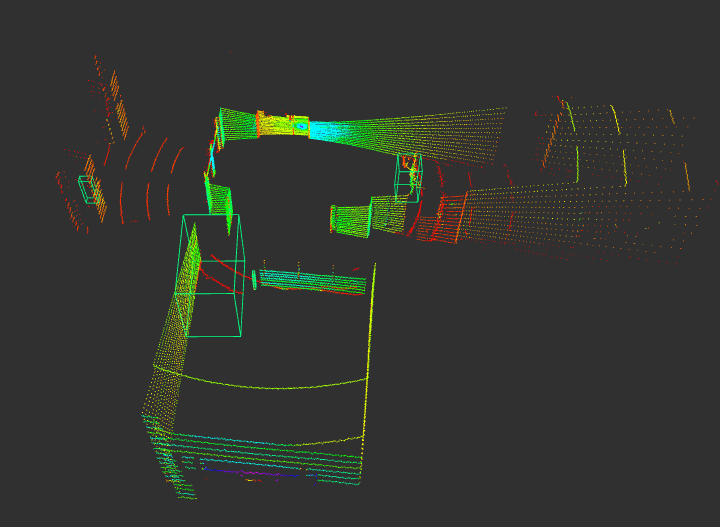
\includegraphics[width=1.0\linewidth]{figures/chap3_fig/onlineSVM/online_train_round3.png}
%     \caption{Online train round 3}
%     \label{Chap3:Fig18}
% \end{figure}

% \begin{figure}[h]
%     \centering
%     % \hspace*{-8mm}
%     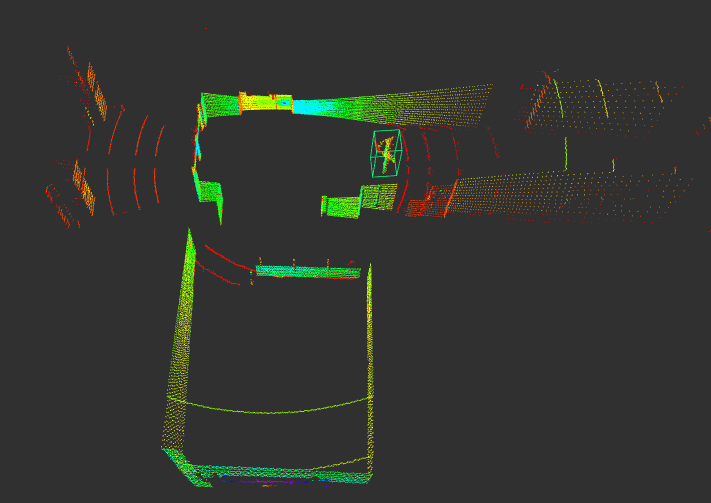
\includegraphics[width=1.0\linewidth]{figures/chap3_fig/onlineSVM/online_train_round5.png}
%     \caption{Online train round 5}
%     \label{Chap3:Fig19}
% \end{figure}

% \begin{figure}[h]
%     \centering
%     \begin{subfigure}{.5\linewidth}
%       \centering
%       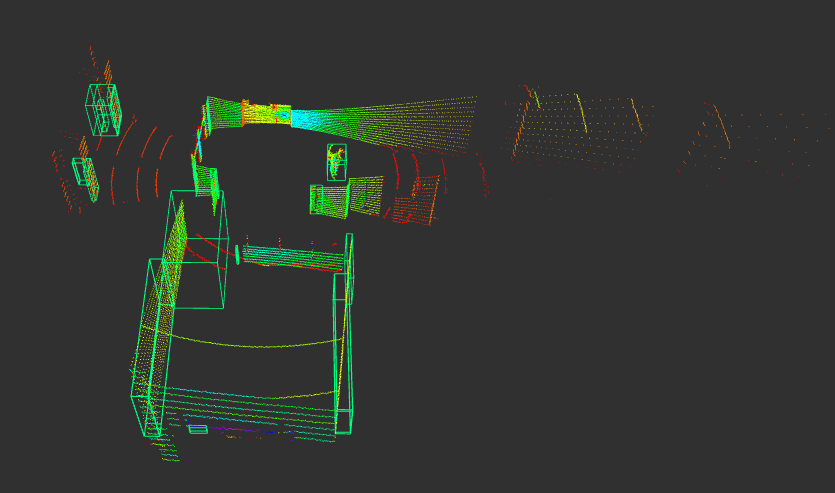
\includegraphics[width=1.0\linewidth,height = 1.0\linewidth]{figures/chap3_fig/onlineSVM/online_train_round1.png}
%     %   \caption{Taking notes with paper \cite{note_paper}}
%       \label{fig:sub1}
%     \end{subfigure}%
%     \begin{subfigure}{.5\linewidth}
%       \centering
%       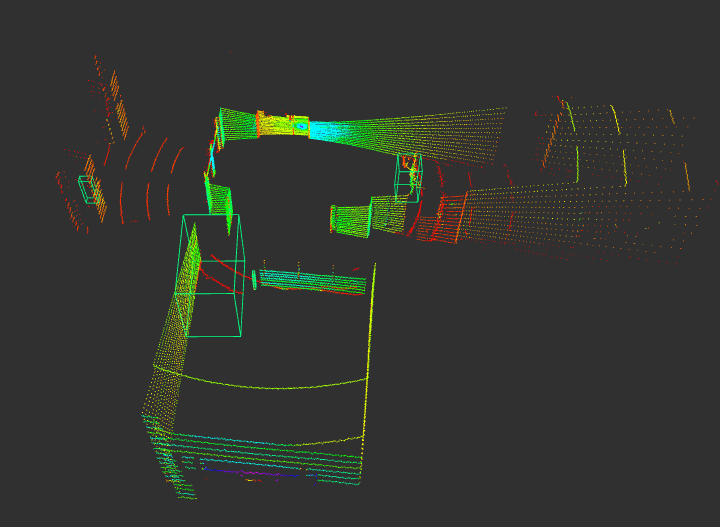
\includegraphics[width=1.0\linewidth,height = 1.0\linewidth]{figures/chap3_fig/onlineSVM/online_train_round3.png}
%     %   \caption{Taking notes with Ipad \cite{note_ipad}}
%       \label{fig:sub2}
%     \end{subfigure}
%     \caption{Icart-mini robot with Velodyne VLP-16}
%     \label{Fig2}
% \end{figure}


\newpage

%------------3.2.4--------------------------------------%
\subsection{PID for Robot controller}
\label{pid_section}

The online learning stage above will yield human cluster's centered position and this data
will be used as input for the PID controller. To successfully follow a human, errors between the
state of robot and human must be diminished to the fullest extent. In actual experiment, z-coordinate of
both human and robot is not essential for the following step. We will only consider offset angle and distance
between the robot and human \cite{refchap2-fig1,DL_Color_feature}, as illustrated in Figure \ref{Chap3:Fig20}.

\begin{figure}[h]
    \centering
    \hspace*{2cm}
    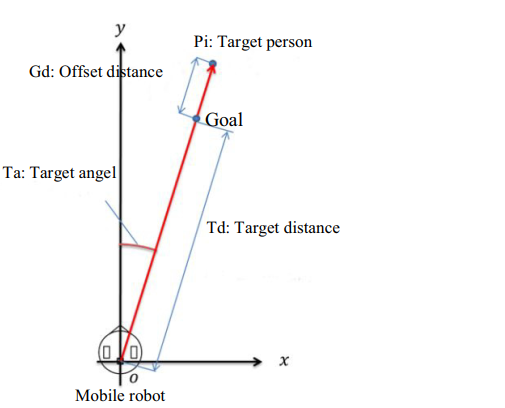
\includegraphics[scale=0.8]{figures/chap3_fig/pid/pid_framework_2.png}
    \caption{Human target distance and direction of mobile robot \cite{hfr_lrs}}
    \label{Chap3:Fig20}
\end{figure}

General offset angle and distance can be determined as in Equation \ref{Chap3:Eq3}. It is
worth noting out that in our case, output human cluster's position is with respect to
the LiDAR sensor's reference frame. In section \ref{Experiments_design_subsection}, one will see that LiDAR and
mobile robot is designed to have same z-axis and same x and y direction. Thus, in 2D format, sensor's frame
coincides with robot's frame and $x_r$ and $y_r$ can be set to zero for simplicity. This equation can
also be used in global coordinate map with tf library \cite{tf_lib} in ROS.

\begin{equation}
    \label{Chap3:Eq3}
    \begin{split}
        d = \quad & \sqrt{(x_h - x_r)^2 + (y_h - y_r)^2} \\
        \theta =  \quad & \taninv {\frac{y_h - y_r}{x_h - x_r}}
    \end{split}
\end{equation}

\newpage

For the following state, PID equation can be used as follows:


% \begin{equation} \renewcommand{\arraystretch}{1.8}
%     \label{Chap3:Eq3}
%     \begin{pmatrix}
%         \dot{x}(t) \\ \dot{y} (t) \\ \dot{z} (t)
%     \end{pmatrix}= K_p \begin{pmatrix}
%         e_x (t) \\e_y (t)\\e_z (t)
%     \end{pmatrix} + K_i \int_{0}^{T} \begin{pmatrix}
%         e_x (t) \\e_y (t)\\e_z (t)
%     \end{pmatrix} \mathrm{dt} + K_d \frac{d}{\mathrm{dt}} \begin{pmatrix}
%         e_x (t) \\e_y (t)\\e_z (t)
%     \end{pmatrix}
% \end{equation}

\begin{equation} \renewcommand{\arraystretch}{1.8}
    \label{Chap3:Eq4}
    \begin{pmatrix}
        v_t \\ \omega_{t}
    \end{pmatrix}=
    \begin{pmatrix}
        \dot{d}(t) \\ \dot{\theta} (t)
    \end{pmatrix}= K_p \begin{pmatrix}
        e_d (t) \\e_{\theta} (t)
    \end{pmatrix} + K_i \int_{0}^{T} \begin{pmatrix}
        e_d (t) \\e_{\theta} (t)
    \end{pmatrix} \mathrm{dt} + K_d \frac{d}{\mathrm{dt}} \begin{pmatrix}
        e_d (t) \\e_{\theta} (t)
    \end{pmatrix}
\end{equation}

with distance error $e_d = (d - D)$ and angle error $e_{\theta} = \theta - \Theta$. They can
also be called as state differences , where $D$ and $\Theta$ are target distance and angle respectively.
In this following step, $D$ is set to be 1m and $\Theta$ is around $5^o$. 3 PID parameters $K_p$ , $K_i$ and $K_d$
are set differently for each testing environment, namely corridor and testing hall (See Chapter \ref{Chap:ExperimentSetup_Results}). These values
are tuned by trial and error until reliable result is attained.

However,to ensure the robot follows the exact
initial person, the position of the human between 2 consecutive detections will be constrained to be no larger
than a maximum distance. We denote $r_t$ as the distance between 2 consecutive recognition and human-filter based velocity is set
as follows:

\begin{equation}
    \label{Chap3:Eq5}
    \begin{split}
        r_t = \quad & \sqrt{({x_h}^t - {x_h}^{t-1})^2 + ({y_h}^t - {y_h}^{t-1})^2} \\
        r_t \leq  \quad &  {v_h}^{max} \Delta t
    \end{split}
\end{equation}

After setting constraints as in Equation \ref{Chap3:Eq5}, target goal or target human's position is fed to the PID
feedback loop as in Equation \ref{Chap3:Eq4} above. This completes the whole process of the proposed pipeline. Final pipeline
result is presented in section \ref{pipeline_result}.

\chapter{Experimental Setup and Results}
\label{Chap:ExperimentSetup_Results}
%---------------------------4.1-----------------------------------%
\section{Experiments Platform}

%-------------------------4.1.1----------------------------------%
\subsection{Experiments Design}
\label{Experiments_design_subsection}

Icart-mini \cite{icart_mini} and VLP-16 LiDAR \cite{vlp16} are the robot and sensor used in this investigation. 
A laptop will be mounted on the robot, it connects to the LiDAR, does 
processing and calculations, and issues orders to the robot. Icart-mini is a 
T-frog robot that has a simple design and can be moved both indoors and outdoors. 
This robot template is available for free. The supplier has offered a variety of 
packages to help users create apps for Icart-mini. Being the smallest in the Velodyne 
product range, the VLP-16 LiDAR scanner, was developed at a low cost with mass 
production in mind, notably for robots, autonomous cars, and industrial automation.

\begin{figure}[h]
    \centering
    \begin{subfigure}{.5\linewidth}
        \centering
        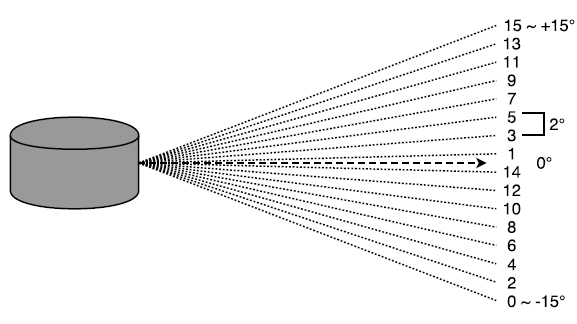
\includegraphics[width=1.0\linewidth,height = 0.5\linewidth]{figures/chap4_fig/Platform/lidar_property.png}
          \caption{LiDAR property \cite{lidarproperties}}
        \label{chap4:fig1:sub1}
    \end{subfigure}%
    \begin{subfigure}{.5\linewidth}
        \centering
        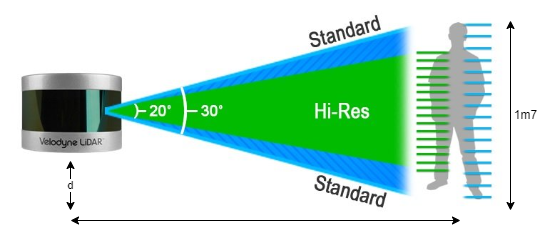
\includegraphics[width=1.0\linewidth,height = 0.5\linewidth]{figures/chap4_fig/Platform/Untitled Diagram-Page-12.drawio.png}
          \caption{Model calculate height of LiDAR \cite{calculateheight}}
        \label{chap4:fig1:sub2}
    \end{subfigure}
    \caption{VLP-16 LiDAR vertical field of view}
    \label{chap4:fig1}
\end{figure}


\begin{table}[h!]
    \centering
    \begin{tabular}{||c|c||}
        \hline
        \rowcolor{lightgray}
        \textbf{Item}                 & \textbf{Specifications}                     \\ [0.5ex]
        \hline\hline
        Scanning rate                 & 10 scans/s                                  \\ \hline
        Horizontal field of view      & $360^o$                                     \\ \hline
        Horizontal angular resolution & $0.23^o$                                    \\ \hline
        Vertical field of view        & $26.8^o$                                    \\ \hline
        Vertical angular resolution   & $2^o$ (16 lines)                            \\ \hline
        Detection range               & 40m for pavement, 120m for cars and foliage \\ \hline
        Range accuracy                & 0.02m                                       \\ \hline
        Wavelength of laser beam      & 905nm                                       \\ [0.5ex]
        \hline
    \end{tabular}
    \caption{3D VLP-16 LiDAR properties \cite{vlp16}}
    \label{Chap4:Table1}
\end{table}


\begin{figure}[!htb]
    \centering
    % \hspace*{-8mm}
    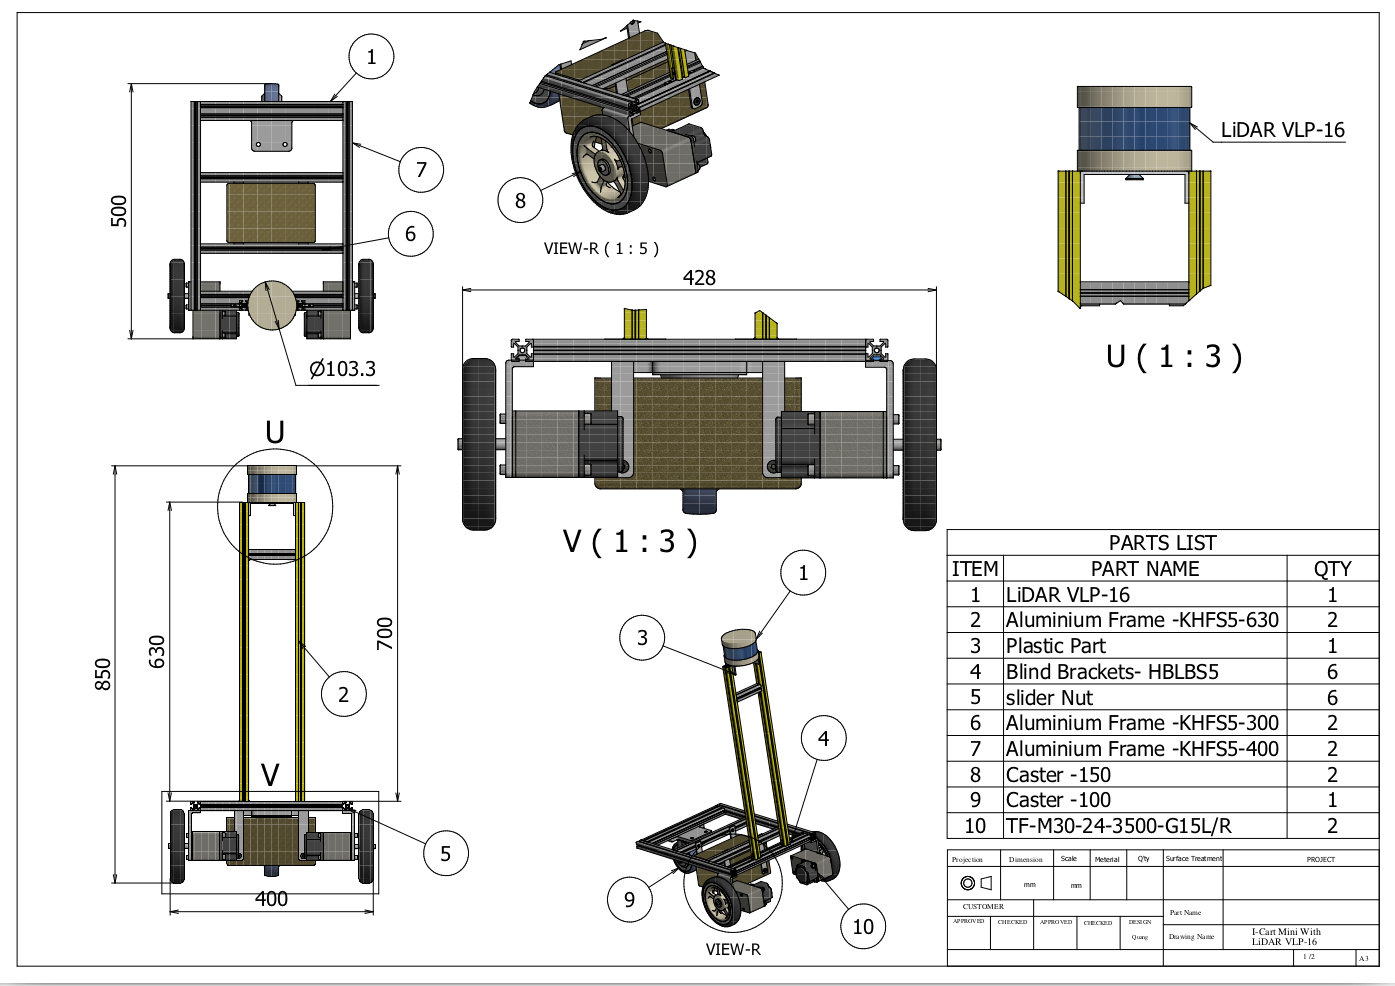
\includegraphics[width=1.0\linewidth]{figures/chap4_fig/Platform/Icart_mini_withLidar_drawing.png}
    \caption{Design of VLP-16 LiDAR onboard Icart-mini robot}
    \label{chap4:fig2}
\end{figure}



\begin{figure}[h]
    \centering
    % \hspace*{-8mm}
    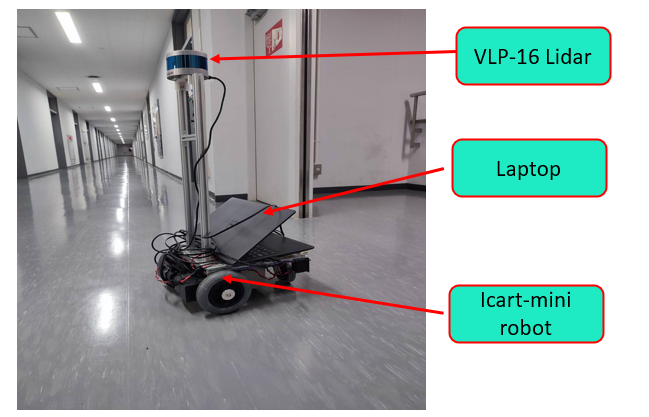
\includegraphics[width=1.0\linewidth]{figures/chap4_fig/Platform/icart_mini_with_lidar.png}
    \caption{Final experiments design in real life}
    \label{Chap4:fig3}
\end{figure}

Figure \ref{chap4:fig1:sub1} and Table \ref{Chap4:Table1}  show the scan properties of 
VLP-16. From these data, one knows that VLP-16 has a total of 16 scans. Each scanning 
ray is aligned at an angle of 2 degrees. The total vertical field of view is 30 degrees. 
The scan range that is considered to be the most detailed will have a scan range of 20 
degrees and a standard of 30 degrees. Consequently, in order to obtain the most complete 
and accurate information about people, we need to place the LiDAR at a certain distance 
from the ground. The height calculation model is shown as Figure \ref{chap4:fig1:sub2} 
below. Assume the minimum distance for the robot to recognize people is at least 2m from 
the robot. The average height of a person is 170cm. From the model, we can calculate 
that the height of the LiDAR will be approximately 80cm from the ground. 
After calculating the required height for the LiDAR, we proceed to fabricate and 
assemble the necessary parts to mount the LiDAR on the robot. The robot model equipped 
with LiDAR is shown in Figure \ref{chap4:fig2}. We used aluminum rods buying from \textit{Misumi}
to connect Icart-mini and VLP-16. The height from the ground to the top of the LiDAR is 
85cm. Figure \ref{Chap4:fig3} displays the full robot model with all of its components. 
A laptop with Ubuntu Operating System will be the processor of the robot. 
In other words, this laptop will be put on top of Icart-mini and acts as the mind of 
the robot. In this laptop, ROS Noetic 20.04 was installed to run the pipeline.


%-------------------------4.1.2----------------------------------%
\subsection{Experiments Setup and Simulations}

In this study, we experimented with the system of robot following people in three 
environments: simulation (Gazebo environment), corridor and hall environment. 
To greatly increase comparability, and make the research project reusable for other
researchers, which indicate that the experiment can be completely recreated without
the necessity to rearrange the real life experiment, we decided to build all
models in Gazebo simulated environment .With the Gazebo environment, it is used to train 
the model, test the PID algorithm and the tracking algorithm.

\begin{figure}[!htb]
    \centering
    % \hspace*{-8mm}
    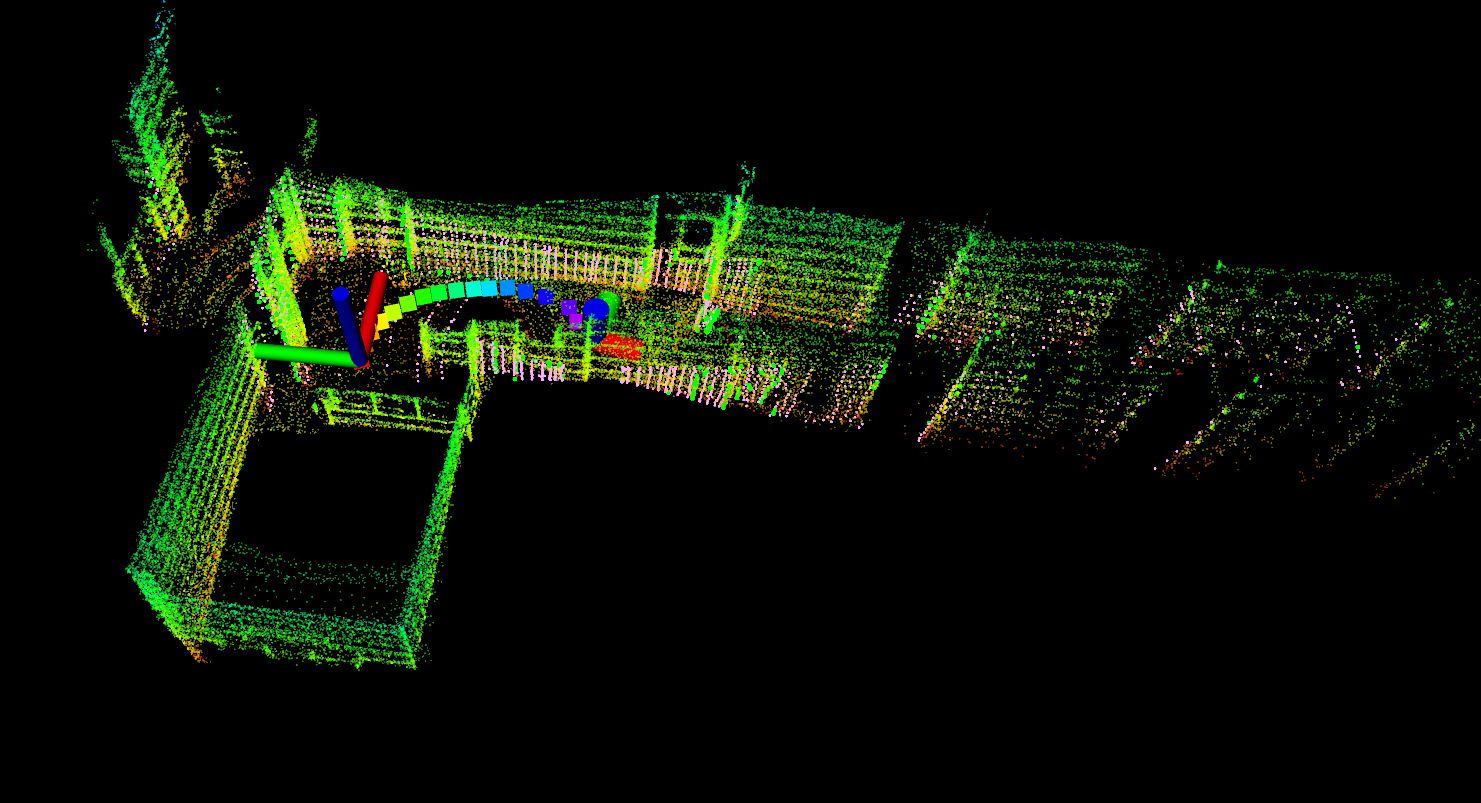
\includegraphics[scale=0.26]{figures/chap4_fig/Platform/Lego-loam-map.png}
    \caption{Corridor 3D Map}
    \label{Chap4:Fig12}
\end{figure}

\begin{figure}[!htb]
    \centering
    % \hspace*{-8mm}
    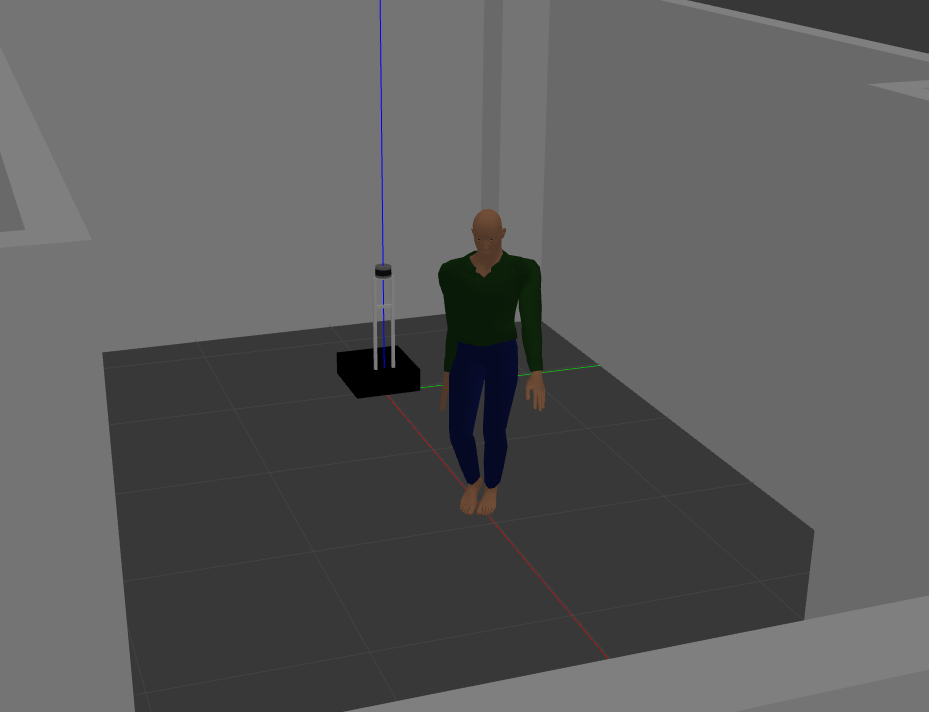
\includegraphics[scale=0.3]{figures/chap4_fig/Platform/human_simulation.png}
    \caption{Human walking simulation using waypoint generator}
    \label{Chap4:Fig11}
\end{figure}

First, for the Gazebo simulation environment, we created an environment 
that was structured like a hallway, which we later used for experiments. In order to 
create the corridor environment as close to reality, we use the ALOAM algorithm 
\cite{legoloam,loam} to scan the corridor area map as illustrated in Figure \ref{Chap4:Fig12}. As we showed in the previous 
workshop, ALOAM is a fairly accurate map scanning algorithm and gives fast results. 
After creating the corridor map, we extracted the images of the map and imported them 
into Gazebo software to create the environment in 1:1 size. In addition, we also added a 
human object environment to train the robot as well as test the algorithm. 
This object will be defined with a certain and repetitive motion trajectory in the environment.
Simulated walking human using waypoint generator is indicated in Figure \ref{Chap4:Fig11}.

\begin{figure}[!htb]
    \begin{subfigure}{.5\linewidth}
        \centering
        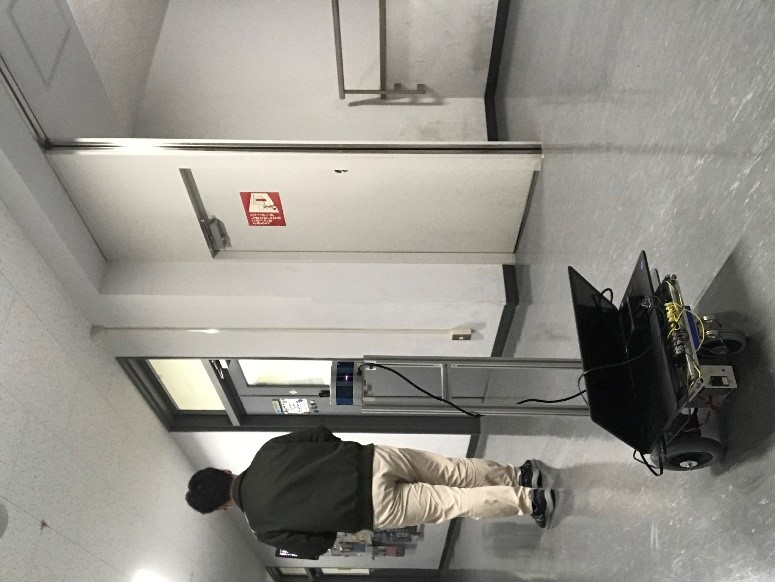
\includegraphics[scale=0.34,angle = -90]{figures/chap4_fig/Platform/corridor_env.jpg}
        \caption{Corridor environment}
        \label{chap4:fig4:sub1}
    \end{subfigure}%
    \begin{subfigure}{.5\linewidth}
        \centering
        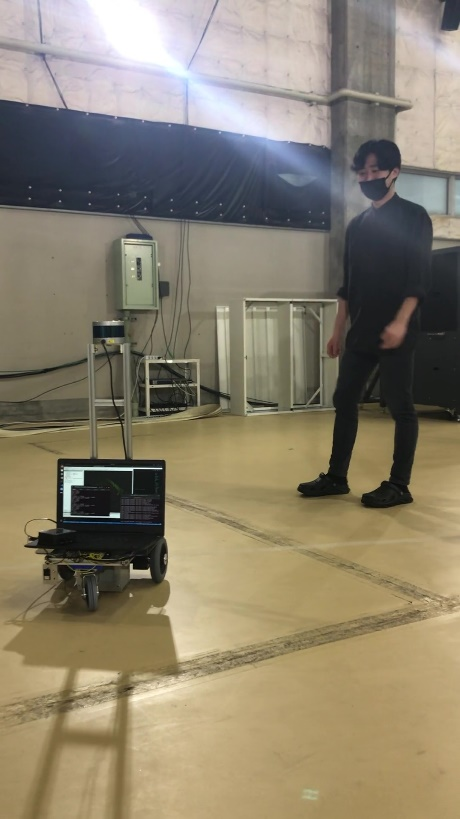
\includegraphics{figures/chap4_fig/Platform/hall_environment.jpg}
        \caption{Testing hall environment}
        \label{chap4:fig4:sub2}
    \end{subfigure}\\[1ex]
    \begin{subfigure}{\linewidth}
        \centering
        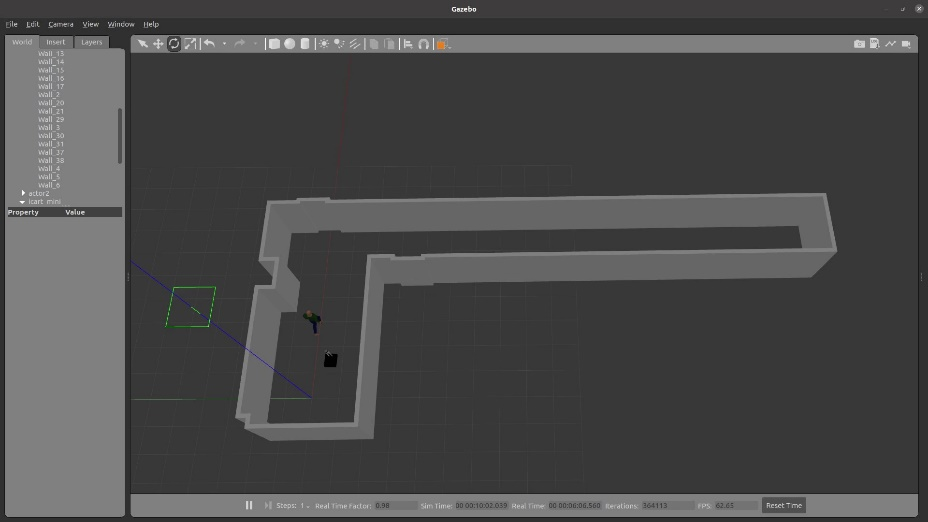
\includegraphics{figures/chap4_fig/Platform/gazebo_environment.jpg}
        \caption{Gazebo environment}
        \label{chap4:fig4:sub3}
        \end{subfigure}
    \caption{Experiment setup in 3 cases}
    \label{Chap4:fig4}
\end{figure}


For experiments conducted in the real environment which includes
the corridor and the aerospace testing hall, robot as in Figure \ref{Chap4:fig3} is 
placed with one participant such as the author himself or author's
friend from laboratory. All experiments are illustrated in Figure \ref{Chap4:fig4}. 
More specifically, Figure \ref{chap4:fig4:sub1} shows the experiment in the corridor, Figure
\ref{chap4:fig4:sub2} shows the experiment in the aerospace testing hall and Figure 
\ref{chap4:fig4:sub3} shows the experiment in the simulated Gazebo environment respectively.

% \newpage
\clearpage

%---------------------------4.2-----------------------------------%
\section{Experiments Results}
\label{Exp_result}

%-----------------------4.2.1-----------------------------%
\subsection{Clustering result}
\label{cluster_result}

This section shows the outcome of point cloud clustering whose method was described in section \ref{Euclidean_cluster_section}.
There are more objects in the aerospace testing hall than in the corridor so the efficiency of the Adaptive clustering technique
is evident in the case of hall environment. For point cloud sets of the same size as a standard human,
we can observe that they are clustered flawlessly without any errors whereas bigger objects in the hall (Figure \ref{Chap3:Fig11})
are sometimes being divided into smaller objects. This is reasonable because their dimensions
belong to various LiDAR's horizontal detected range. Walls in the corridor also behave in the similar 
way, as shown in Figure \ref{Chap3:Fig13}. 

\begin{figure}[h]
    \centering
    % \hspace*{-8mm}
    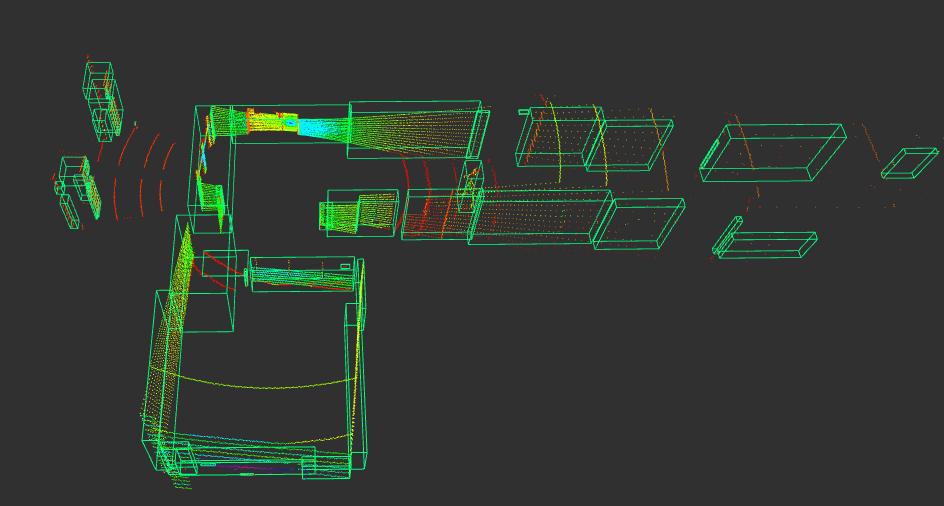
\includegraphics[width=1.0\linewidth]{figures/chap3_fig/euclidean/3_2_7.png}
    \caption{Corridor clustering result}
    \label{Chap3:Fig13}
\end{figure}

\begin{figure}[h]
    \centering
    % \hspace*{-8mm}
    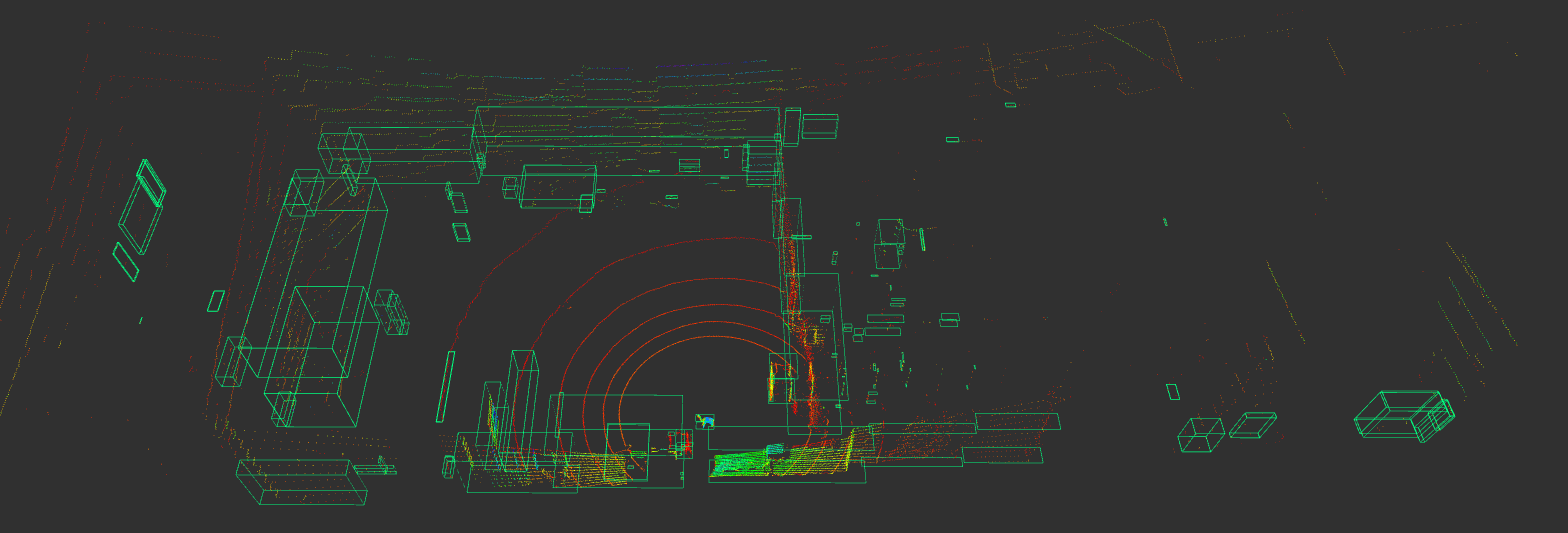
\includegraphics[width=1.0\linewidth]{figures/chap3_fig/euclidean/3_2_5.png}
    \caption{Testing hall clustering result}
    \label{Chap3:Fig11}
\end{figure}

Some objects which are outside the window and not inside the 
corridor are even clustered because of the wide detection range of VLP-16 LiDAR. Those objects are split into multiple smaller 
clusters because they are too far away from the sensor,however, it is not a main issue of the clustering method. This is because 
in this research the distance between human and robot is constrained to be not larger than a maximum value (see section \ref{pid_section}) to 
ensure that human is always clustered into only one cluster and also the inaccuracy of the classification will reduce greatly. Hence, as long as 
human is clustered correctly, this cluster will be treated as positive samples for the next onlin training step. To sum up ,it is appropriate to assert that 
the performance of the adaptive Euclidean clustering in this HFR experiment is acceptable.

% \clearpage



%-----------------------4.2.2-----------------------------%
\subsection{Online training for SVM result}
\label{online_svm_result}

This section displays the consequence of online training whose method was detailed in 
section \ref{online_learning_section}. This training can either be done in two ways: by directly training with robots or by 
recording point cloud into \textit{bag} file and then train later. Both ways will still generate the same result as in 
Figure \ref{Chap4:Fig23}. The result of the online training result can be analysed as follows. First, the SVM human classifier is trained
with a small initial training dataset and shows a poor classification result as in Figure
\ref{Chap4:Fig23:sub1}. After that, the P-N generator will correct wrong samples as described in section 
\ref{online_learning_section} and retrain the whole classifier for better classification result. Then in round 3, we 
can observe from Figure \ref{Chap4:Fig23:sub2} that now there are only 2 clusters are being classified incorrectly as human. When the 
final training round (round 5) is reached, there are no more mis-classified clusters and human cluster is correctly classified, as indicated 
in Figure \ref{Chap4:Fig23:sub3}.

\begin{figure}[!htb]
    \begin{subfigure}{1\linewidth}
        \centering
        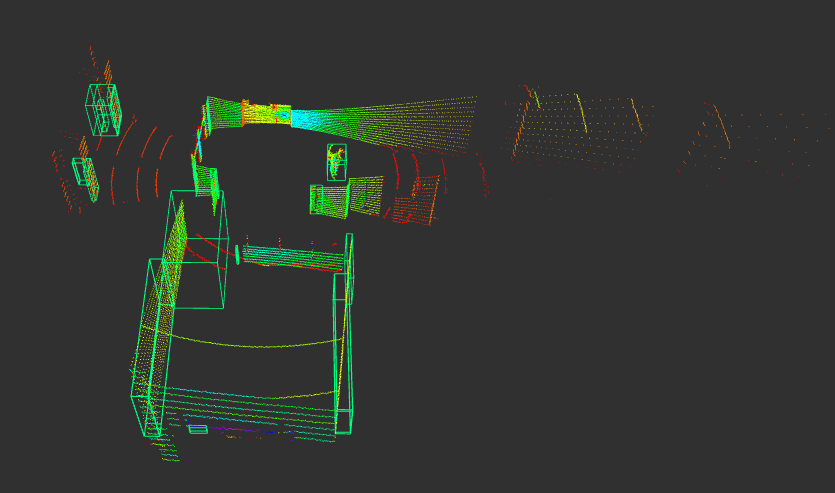
\includegraphics[scale=0.3]{figures/chap3_fig/onlineSVM/online_train_round1.png}
        \caption{Online train round 1 (initial)}
        \label{Chap4:Fig23:sub1}
    \end{subfigure}
    \begin{subfigure}{1\linewidth}
        \centering
        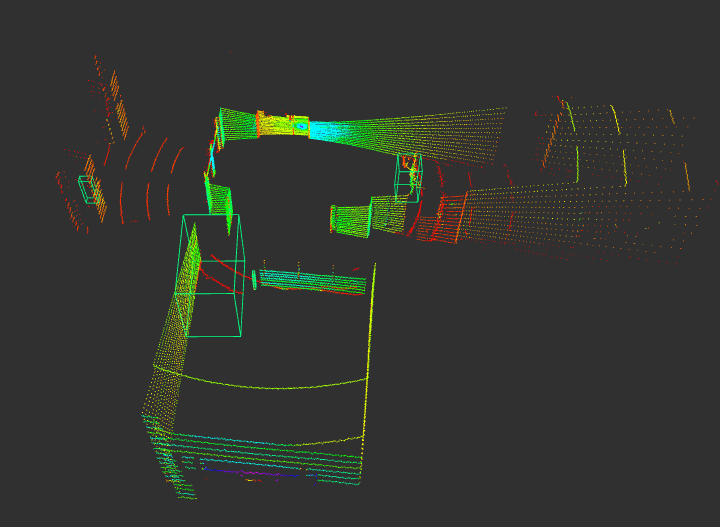
\includegraphics[scale=0.348]{figures/chap3_fig/onlineSVM/online_train_round3.png}
        \caption{Online train round 3}
        \label{Chap4:Fig23:sub2}
    \end{subfigure}
    \begin{subfigure}{1\linewidth}
        \centering
        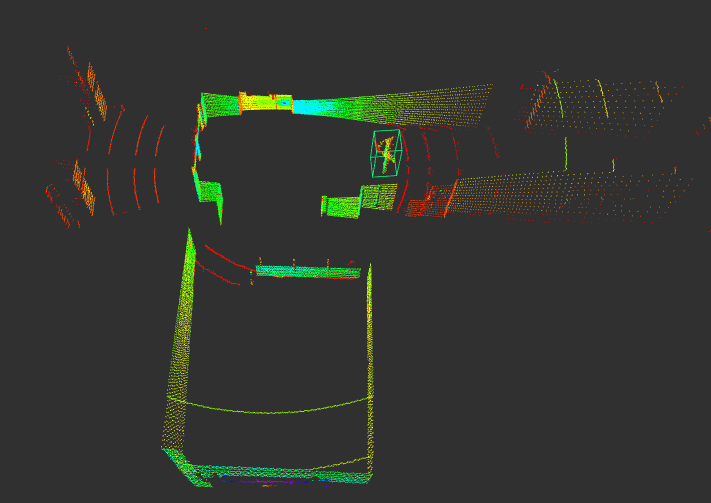
\includegraphics[scale=0.35]{figures/chap3_fig/onlineSVM/online_train_round5.png}
        \caption{Online train round 5}
        \label{Chap4:Fig23:sub3}
    \end{subfigure}
    \caption{Online training result in corridor environment}
    \label{Chap4:Fig23}
\end{figure}

% \begin{figure}[h]
%     \centering
%     % \hspace*{-8mm}
%     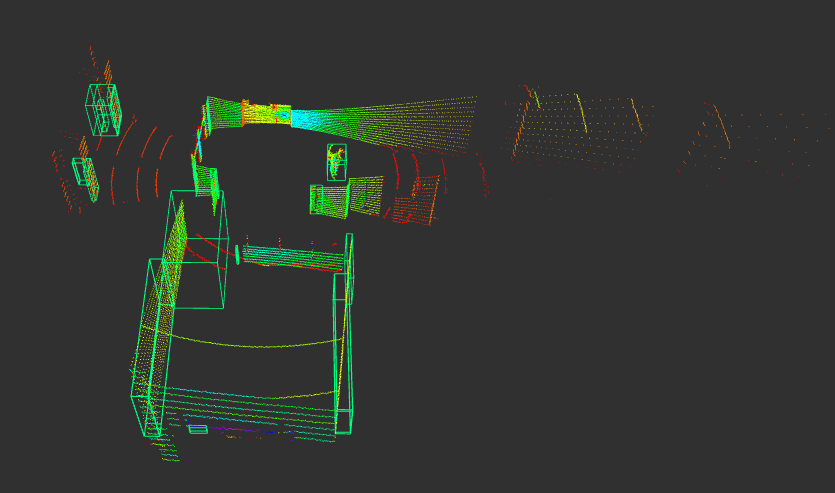
\includegraphics[scale=0.5]{figures/chap3_fig/onlineSVM/online_train_round1.png}
%     \caption{Online train round 1 (initial)}
%     \label{Chap3:Fig17}
% \end{figure}

% \begin{figure}[h]
%     \centering
%     % \hspace*{-8mm}
%     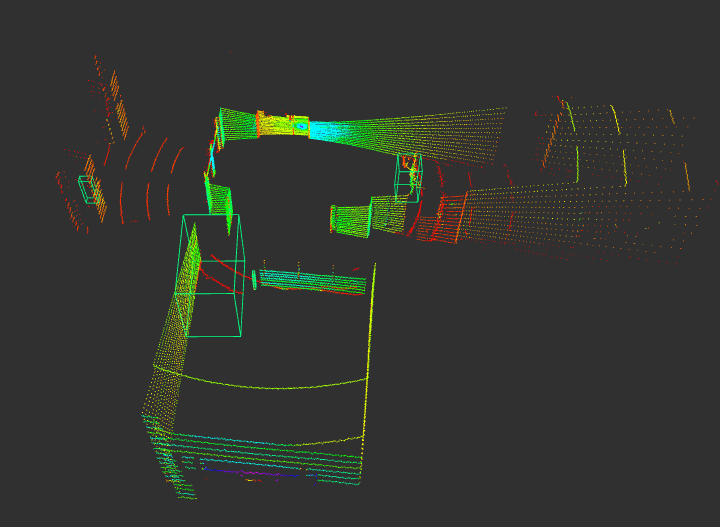
\includegraphics[width=1.0\linewidth]{figures/chap3_fig/onlineSVM/online_train_round3.png}
%     \caption{Online train round 3}
%     \label{Chap3:Fig18}
% \end{figure}

% \begin{figure}[h]
%     \centering
%     % \hspace*{-8mm}
%     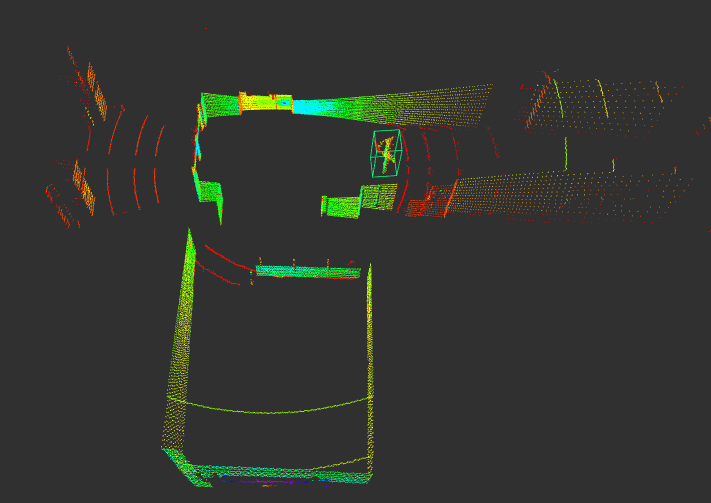
\includegraphics[width=1.0\linewidth]{figures/chap3_fig/onlineSVM/online_train_round5.png}
%     \caption{Online train round 5}
%     \label{Chap3:Fig19}
% \end{figure}

It is worth noting that the result of the online human classifier is mainly affected by the decision of 
the P-expert and N-expert of the generator in the online learning framework. As long as all assumptions and conditions such as 
human-like trajectory and static objects mentioned in section \ref{online_learning_section} are still satisfied, online human classifier
will perform effectively as in Figure \ref{Chap4:Fig23}.

%there are stacked floating elements, such as tables or figures, they will be flushed out before starting the new page.
\clearpage

%-----------------------4.2.3-----------------------------%
\subsection{Pipeline testing result}
\label{pipeline_result}

This section demonstrates the testing result of the whole pipeline whose image was shown in section \ref{whole_pipeline_intro}.

\begin{figure}[!htb]
    \centering
    % \hspace*{-8mm}
    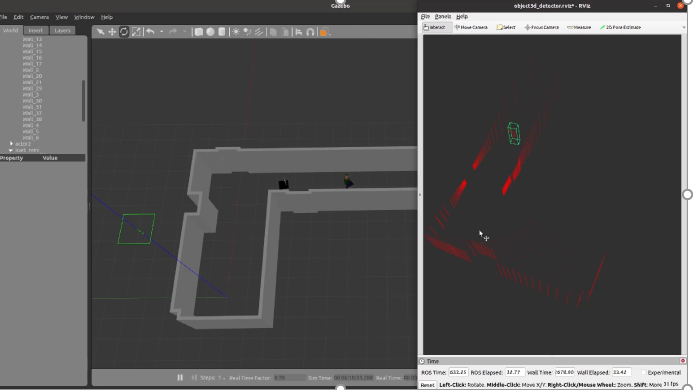
\includegraphics[scale=0.8]{figures/chap4_fig/Results/Gazebo/gazebo_simulation_result.png}
    \caption{Pipeline testing in Gazebo environment}
    \label{Chap4:fig22}
\end{figure}


\begin{figure}[!htb]
    \centering
    % \hspace*{-8mm}
    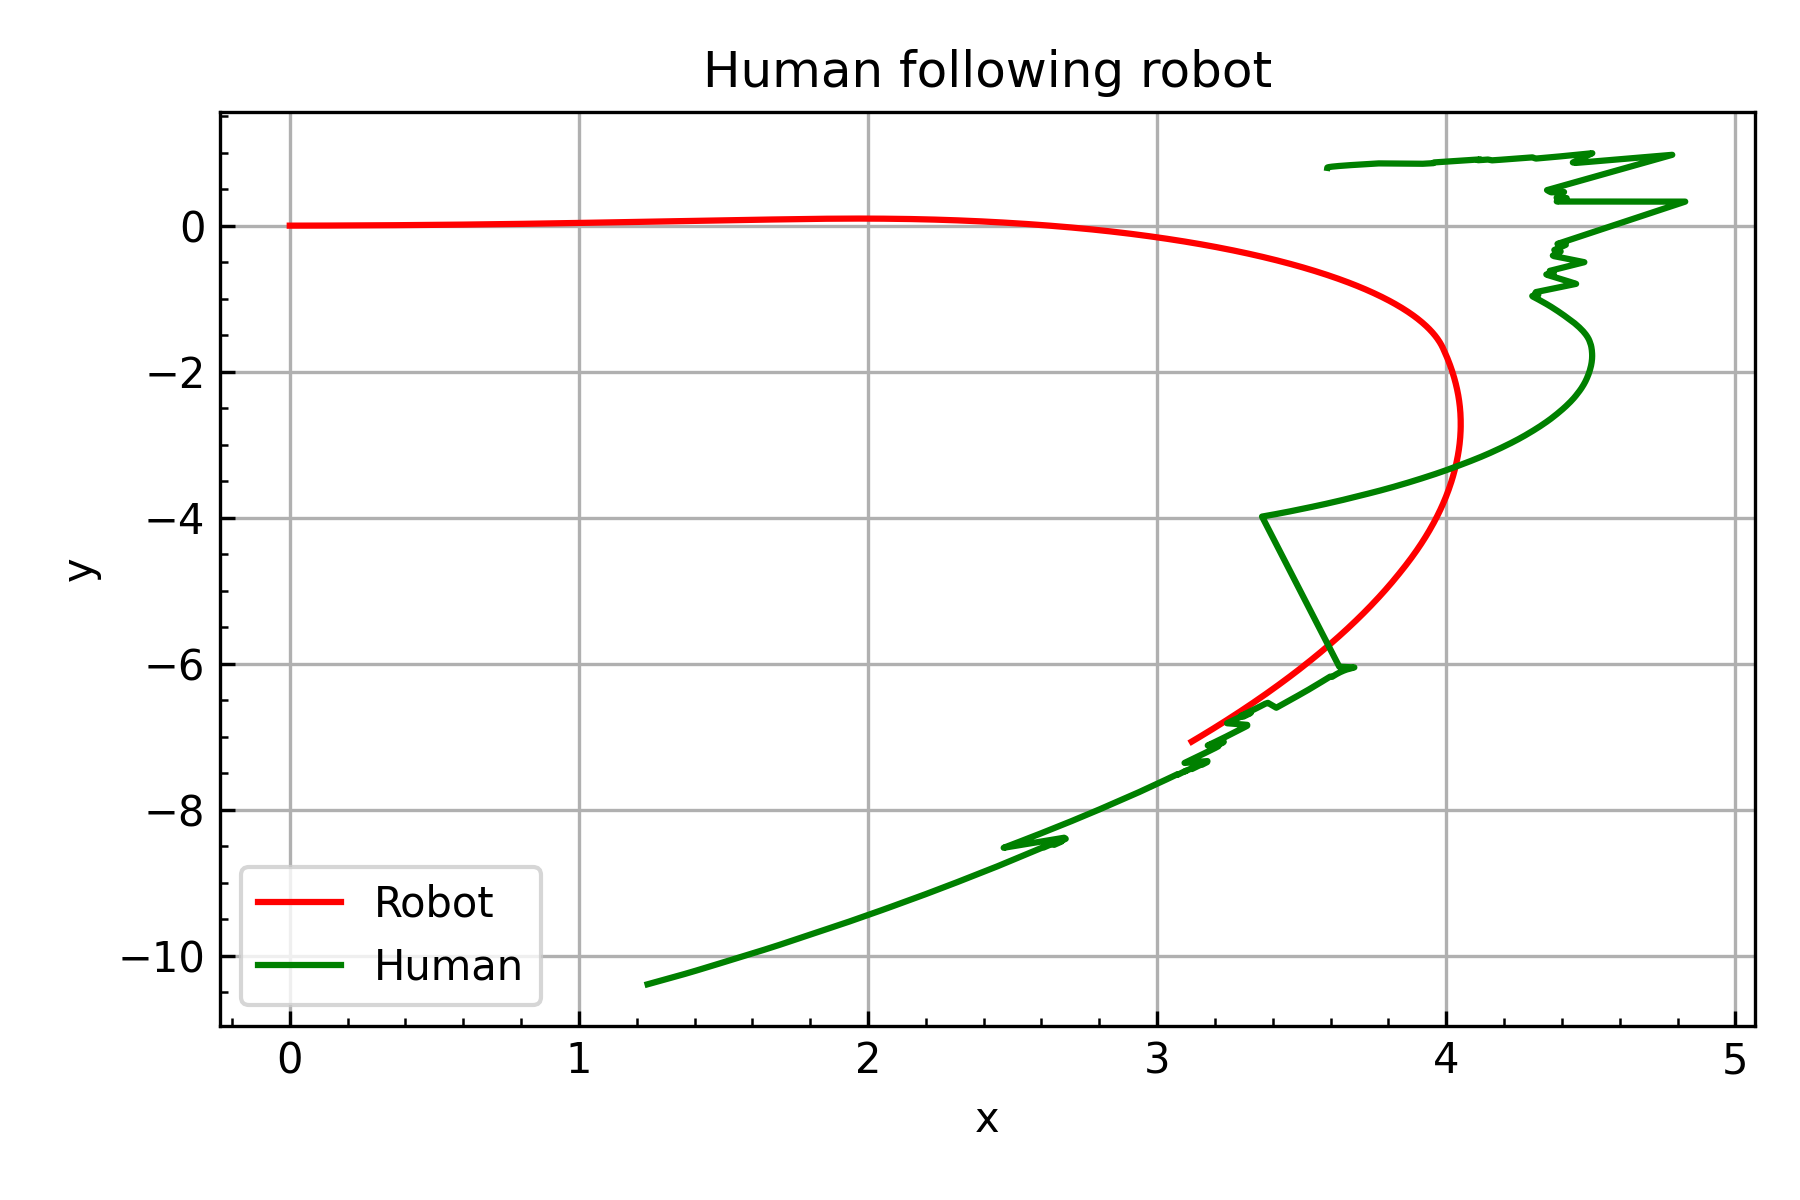
\includegraphics[scale=0.8]{figures/chap4_fig/Results/human_following_robot_gazebo_4.png}
    \caption{HFR 2D path in Gazebo simulated environment}
    \label{Chap4:Fig7}
\end{figure}

\begin{figure}[!htb]
    \centering
    \begin{subfigure}{.5\linewidth}
        \centering
        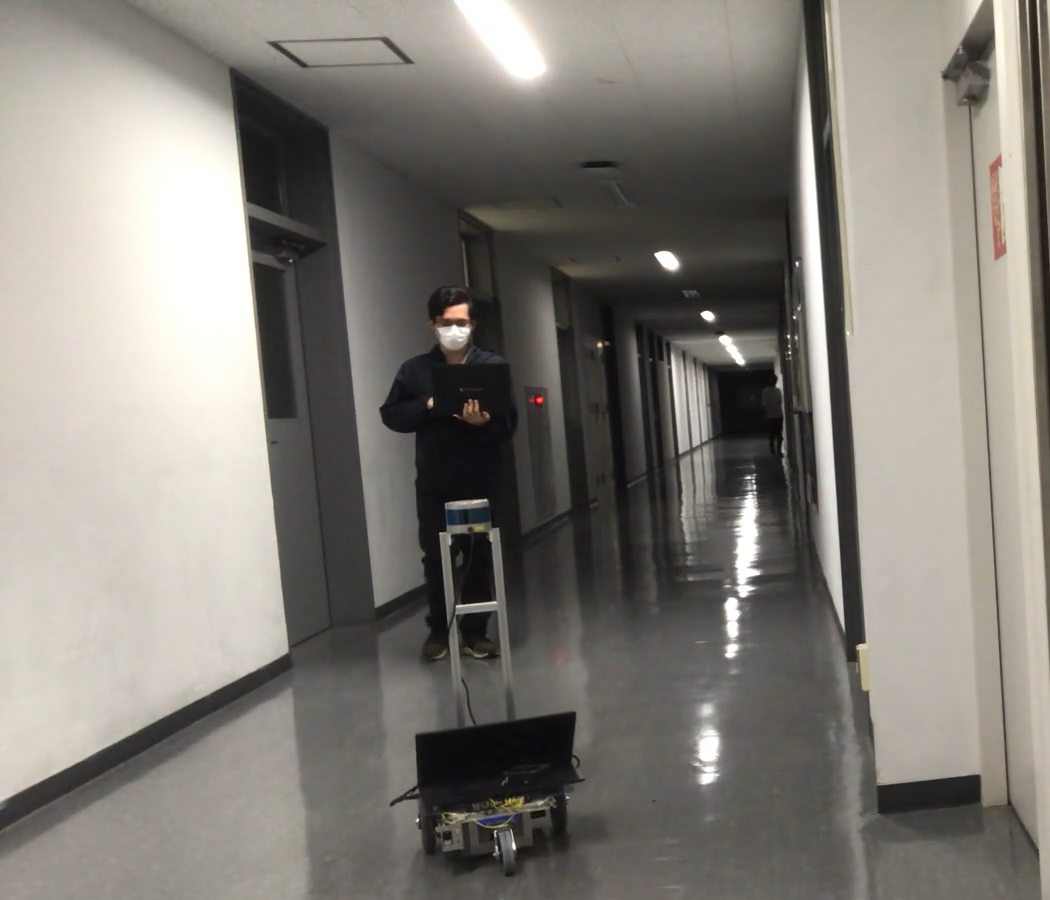
\includegraphics[width=0.9\linewidth,height = 1.0\linewidth]{figures/chap4_fig/Results/Corridor/real_corridor.png}
          \caption{HFR in real corridor}
        \label{chap4:fig20:sub1}
    \end{subfigure}%
    \begin{subfigure}{.5\linewidth}
        \centering
        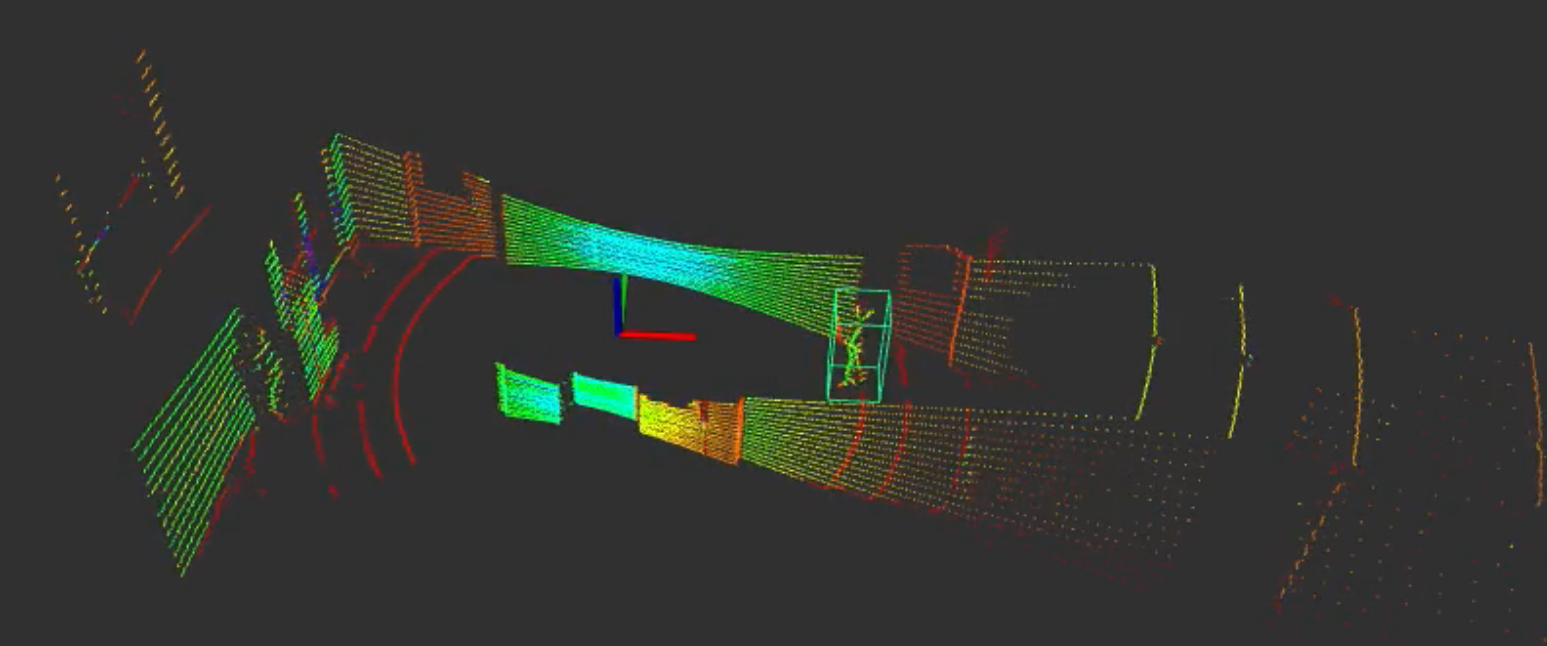
\includegraphics[width=1.0\linewidth,height = 1.0\linewidth]{figures/chap4_fig/Results/Corridor/rviz_corridor.png}
          \caption{Corresponding time in Rviz}
        \label{Chap4:fig20:sub2}
    \end{subfigure}
    \caption{Pipeline testing in corridor environment}
    \label{Chap4:fig20}
\end{figure}

\begin{figure}[!htb]
    \centering
    \hspace*{-2cm}
    \includegraphics[scale=0.8]{figures/chap4_fig/Results/human_following_robot_corridor_5.png}
    \caption{2D path in Nagoya University Engineering Building 2 4th floor corridor}
    \label{Chap4:Fig8}
\end{figure}


\begin{figure}[!htb]
    \centering
    \begin{subfigure}{.5\linewidth}
        \centering
        \includegraphics[width=0.95\linewidth,height = 0.5\linewidth]{figures/chap4_fig/Results/Hall/real_hall.png}
          \caption{HFR in Testing hall}
        \label{chap4:fig21:sub1}
    \end{subfigure}%
    \begin{subfigure}{.5\linewidth}
        \centering
        \includegraphics[width=0.95\linewidth,height = 0.5\linewidth]{figures/chap4_fig/Results/Hall/rviz_hall.png}
          \caption{Corresponding time in Rviz}
        \label{Chap4:fig21:sub2}
    \end{subfigure}
    \caption{Pipeline Test in aerospace hall environment}
    \label{Chap4:fig21}
\end{figure}


\begin{figure}[!htb]
    \centering
    % \hspace*{-8mm}
    \includegraphics[scale=0.8]{figures/chap4_fig/Results/human_following_robot_hall_6.png}
    \caption{2D Path in Nagoya University ‘s Aerospace Testing hall}
    \label{Chap4:Fig9}
\end{figure}

% \begin{figure}
%     \begin{subfigure}{.5\linewidth}
%         \centering
%         \includegraphics{figures/chap3_fig/onlineSVM/online_train_round1.png}
%         \caption{a}
%         \label{chap10:fig4:sub1}
%     \end{subfigure}%
%     \begin{subfigure}{.5\linewidth}
%         \centering
%         \includegraphics{figures/chap3_fig/onlineSVM/online_train_round3.png}
%         \caption{}
%         \label{chap10:fig4:sub2}
%     \end{subfigure}\\[1ex]
%     \begin{subfigure}{\linewidth}
%         \centering
%         \includegraphics{figures/chap3_fig/onlineSVM/online_train_round5.png}
%         \caption{}
%         \label{chap10:fig4:sub3}
%         \end{subfigure}
%     \caption{Experiment setup}
%     \label{chap10:fig4}
% \end{figure}
\clearpage

Figure \ref{Chap4:fig22} and \ref{Chap4:Fig7} show the pipeline testing result in 
the Gazebo simulated environment. Figure \ref{Chap4:fig20} and Figure 
\ref{Chap4:Fig8} illustrate the result in the corridor while Figure \ref{Chap4:fig21} and Figure \ref{Chap4:Fig9} show the result 
in the testing hall respectively. In particular, each pair of these Figures first provides the following result in each environment with its corresponding time in Rviz (ROS Visualiation) in the first figure 
and manifests the path of both robot and human in the 2D plane in the second figure. Rviz image describes the human detection part of the pipeline by surrounding human body 
with a green box in each frame. The 2D plot describes the tracking and following part of the pipeline with green path for human and red path for robot.
In Gazebo simulation case, the robot can detect the simulated walking human and follow human's trajectory in the simulated corridor. In this simulation, we only made the human 
walk in a straight path then turn right at the corner and then go straight again. The robot follows him and creates a red curve as in Figure \ref{Chap4:Fig7}. We can observe that
the detection is not good in the simulated case with many lost target moments expressed by a green large zigzag and squiggly line. This is because the LiDAR's intensity simlation in Gazebo is not similar as in 
real life and in SVM classification, it requires 27 dimensions of LiDAR reflection intensity (see Table \ref{Chap3:Table1}) to train the human model. In fact, simulating LiDAR intensity is still complicated and demands more research work in the future.
However, despite that, the inaccuracy of human detection algorithm in the simulated case does not affect the following process because in the PID step we have added the human based velocity filter so that even the robot losts human target or misclassifies human in 
some frames, the robot can still re-find human in next frame and follow human smoothly. This happens in both other cases, in the corridor and in the testing hall. In the 
case of the corridor, the human even tried to change the direction of movement continuously, from left to right then from right to left and so on. The robot followed him smoothly and 
generated a red curve that is almost identical in shape to the human's green trajectory, as indicated in Figure \ref{Chap4:Fig8}. 
In the hall case, the robot even detected and followed the human and made a close loop path as in Figure \ref{Chap4:Fig9}. This confirms that the pipeline works well in both corridor case and testing hall case. 
The robot can still find the person even when the robot misclassifies other objects during the following process. We also notice that the robot's route is a red smooth curve while human's path is a rough green curve in all 3 cases. 
The reason for that is because the robot's path is directly calculated by its wheel encoder whereas evaluating human's position in each frame took time to operate and transfer to the global coordinate. In all 3 test cases, we make the assumption that 
there are not any obstacles that can prevent the robot from following human. This is a drawback of this pipeline and will be discussed in Chapter \ref{Chap:Conclusion_FutureWork}.

\chapter{Conclusions and Future Work}
\label{Chap:Conclusion_FutureWork}
\section{Summary and Conclusion}
\label{summa_conc}

% \textcolor{red}{
% It would be better what each chapter has the same volume of information, i.e., numbers of pages have to be close.
% However, I know it is not easy to write much information at the conclusion.
% But, You need to write 2 or 3 pages at least.
% For example, please write \\
% - Why did you choose this research \\
% - What was the problem and motivated you to conduct the research \\
% - What types of proposal was required \\
% - How did you overcome the problems in terms of technologies \\
% - How you could confirm effectiveness of the proposal \\
% - and so on \\
% }
Making robots that follow people is one of the most exciting uses of robotics. 
Long-term development can be done from there to provide other uses. At the moment, 
there are few studies on employing robots to track a single object, and these studies 
have mixed results.
The bulk of problems with monitoring people or objects nowadays, in particular, 
use cameras to collect data. It is simple to lose track of things due to the camera's 
still constrained information-collection range and limitations in many complex 
environmental situations. I decided to choose HFR system development as my thesis topic 
as a result of these factors. My study for a graduation project specifically researches 
for the employment of a 3D LiDAR user-following robot system.\\

There are several challenges in the study process because there have not been many studies targeting at 
utilizing 3D LiDAR to identify and track individuals. In contrast to utilizing a 
camera, 3D LiDAR finds fewer characteristics in RGB or RGB-D pictures, making it 
more difficult to identify humans. We had trouble locating and choosing 
characteristics that can be employed in the robot system that follows people 
comparing to using camera in the development of the point-cloud 
user recognition algorithm since not all characteristics that are calculated using 
collected point-clouds are useful. Because that feature does not yet exude 
quiet, some algorithm will lengthen calculation times and some will produce noise during the detection. 
The outcomes of training and testing are also poor since there is no environment 
and training data. We have not been able to test in scenarios with more complexity. 
Even if there are still many obstacles to overcome, we continue to work on 
finishing the research since it is a promising and novel area that requires 
further study in order to be effectively applied to human life.\\

The HFR system with 3D LiDAR is proposed in the thesis, with the 3 key components 
being SVM (online learning) for human tracking and detection, human filter based velocity as well as 
PID control for guiding the robot to the user's position.
We based on earlier research for the human identification and tracking section, 
which uses online learning and a tracker to be able to spot individuals moving. 
In order to increase the accuracy of persons detection, we also introduced a new 
feature which is the volume feature to the SVM model.\\

We have added RANSAC, which removes the point-cloud as a plane, and a boundary filter, 
which is the ROI around the robot, before the human identification section in 
order to increase the processing performance for the online learning in a certain time 
period. In specific, only everything within 10 meters of the robot should be taken into account and we
remove any extraneous objects from the ROI area. Both actions can save processing time and 
eliminate noise. We tested the HFR pipeline in 3 different
environments (Gazebo environment, university's corridor, and testing hall) and this
pipeline performed well enough in all testing cases.\\



% The robot can still find the person even when the robot misclassifies other objects
% during the following process.
% However, there are some weak points in this pipeline that needs to solve in the future:

% \begin{enumerate}
%     \item Robots can only follow the human position without avoiding obstacles
%     \item If the environment has multiple people, especially when people are standing
%           close to each other as groups, the robot can not distinguish which person to follow

% \end{enumerate}

Our study still has some limitations because of the limited research time 
and the lack of expertise and understanding in robotics. Robots can only follow 
people at the moment and they are also unable to go around barriers. In other words, 
robots can only follow the human position without avoiding obstacles and if the environment has multiple people, especially when people are standing
close to each other as groups, the robot can not distinguish which person to follow.
The robot's movement is still fairly sluggish, and it does not react strongly 
to objects that move quickly, particularly in areas with plenty of people and 
items arranged side by side. If they are too close together, single items in 
online learning are difficult to distinguish. 

\newpage

\section{Future Work}
\label{future_work}

Since the HFR system employing 3D LiDAR still has numerous limitations, more study 
into this area may be beneficial. By integrating 3D LiDAR with the camera, 
for instance, it is easier to recognize several individuals standing near to 
one another or people standing next to another item. LiDAR offers precise 3D 
geometry, whereas cameras record additional contextual data 
\cite{fusionlidarandcamera}. In short, we want to fuse other sensors to add more necessary features and better deal with challenging situations such as groups
mentioning in section \ref{summa_conc}.\\

With regards to the issue of navigation and control, the research still only 
uses a basic PID algorithm to move the robot to a person's position. 
To avoid colliding with, harming, or hurting the surrounding environment or the 
robot itself, the robot must be able to avoid obstacles in the fully autonomous 
problem. As a result, the intergration of algorithms such as A*, D*, RRT, 
and others \cite{lspathplanning} should be researched in order to improve and enhance the 
HFR system in addition to obstacle avoidance. In other words, research works require combining obstacles avoidance to make the robot follow the human more efficiently.\\

In the realm of control, PID is still a reliable and straightforward control 
algorithm. The study's findings, however, show that PID is still not particularly 
adept at tracking individuals. The future research can utilize MPC instead of PID 
to follow the path from the robot to the location of the human without the robot 
following straight to the position of the person as in the current study since 
MPC has numerous notable benefits over PID \cite{comparepidmpc}.

% Fuse other sensors to add more necessary features to better deal with challenging situations such as groups




% the \appendix tag tells LaTeX where it should start labelling chapters with letters (denoting appendices) rather than numbers (denoting main chapters)
% \appendix 

% \chapter{Appendix title (if needed)}
% An Appendix is offered for complementary tables, graphs, code, etc.

% \chapter{}
% An extra Appendix is offered for complementary tables, graphs, code, etc. 

Appendices can be added or deleted from the document by using the \textit{$\backslash$ input} command in the MainDocument.tex file.

% \bibliographystyle command to choose the format of your bibliography. More examples of bibliography styles can be found at https://www.overleaf.com/learn/latex/Bibtex_bibliography_styles
% \bibliographystyle{unsrtnat}

% \bibliography is the command for the actual file containing your bibliographic data. This file can be produced manually or automatically using software such as BibTeX. Both options can work, however, learning to use BibTex is beneficial in the long run. An example of the format needed to generate your own bibliography file can be found as the bibliography.bib file here provided.

% \bibliography{mybib}

%   \nocite{*}
%   \printbibliography %Prints bibliography

\chapter{Acknowledgements}

In the process of writing this thesis, I have received a great deal of support and assistance.
I would first like to thank my supervisors, Professor Naoki Akai and Professor Susumu Hara,
whose expertise was invaluable in the formulating of the research topic and methodology
in particular. Professor Hara, thank you for giving me a valuable opportunity to study and research in your lab as an undergraduate researcher. Professor Akai, thank you for introducing me to ROS, guiding me in my first tentative steps in the Linux world and have helped develop a stronger desire to continue to pursue research in the robotics field.

I would love to thank my family in Vietnam, especially my father - Quan Le, my mother - Thinh Tran and my sister - Ha Le, for always supporting 
me whenever I need throughout this journey. 
I would love to thank my senpai - Truong Phan, 
for his continuous guidance and support during my 4 years at 
Nagoya University. I would also love to thank my kouhai - 
Thanh Nguyen for helping me filming my experiments. Finally, 
I would like to thank all lab colleagues and seniors in the 
laboratory, especially the ARIC team with Arashi-san, Yasui-san and Kane-san.
% \afterpage{\blankpage}

\chapter{References}
\nocite{*}
\printbibliography[heading=none]

\end{document}
